\documentclass[12pt]{article}
\usepackage[english]{babel}
\usepackage[
    letterpaper,
    top=1.7cm,
    bottom=1.7cm,
    left=2.5cm,
    right=2.5cm
]{geometry}

\usepackage{lib/main}
\usepackage{lib/commands}
\usepackage{booktabs}
\definecolor{backcolour}{rgb}{0.95,0.95,0.95}

\title{Meta-Learning Metaprogram Primitives for \\ Program Induction on List Manipulation Tasks}
\author{Yiding `Vincent' Song, Christopher Bates, Kazuki Irie, Samuel Gershman}
\date{\today}

\begin{document}

\maketitle

\begin{abstract}
    Program induction represents an important skill in abstracting away from observations to explaining them with programs, believed to enable faster concept-learning and generalisation in humans.
    Traditionally, efforts at eliciting such capabilities in machines have been achieved through a variety of neuro-symbolic methods.
    However, given the success of meta-learning frameworks on systematic generalisation \citep{lake2023human}, we propose to study program induction through a meta-learning framework instead.
    Our preliminary results demonstrate that Transformers can learn to perform program induction on list-manipulation tasks, with meta-learning boosting accuracy in data-limited settings.
    Meanwhile, regardless of dataset size, meta-learned models tend to form representations that align more closely to metaprogram primitives (`metaprimitives') than their in-weight counterparts.
    This suggests that meta-learning encourages Transformers to develop qualitatively different algorithms to program induction problems, potentially favouring metaprimitive-related solutions that have been shown to be effective symbolic models of human behaviour \citep{rule2024symbolic}.
\end{abstract}

\section{Introduction}
\label{sec:introduction}

Systematic generalisation is the ability to understand and produce novel concepts by recombining known ones. It is an important cognitive ability in humans for generating a rich and structured representation of the world, and has been a heavily studied topic for neural networks in recent machine learning literature \citep{drozdov2023compositional, kim2020cogs, lake2018generalization, lake2023human, liang2024diffusion}. In particular, the work of \citet{lake2023human} gave the first empirical demonstration that neural networks can meta-learn to generalise systematically in a human-like way, where a Transformer {\it learns to learn} compositionality through a diverse series of training examples.

We are interested in the dual but more complex problem of program induction. More specifically, let $F$ be a set of existing functions available to the model. Systematic generalisation requires models to correctly predict $\vec{y} = f(\vec{x})$ on a given function $f: X \to Y$ and input $\vec{x} \in X$, where $f$ is a novel composition of functions in $F$, and the input $\vec{x}$ and output $\vec{y}$ lie in some input and output space $X, Y$ respectively. Meanwhile, given a set of input-output (I/O) pairs $D \subset X \times Y$, program induction asks the model to {\it find} a novel composition $\hat{f}: X \to Y$ such that $\vec{y} = \hat{f}(\vec{x})$ for all $(\vec{x}, \vec{y}) \in D$.

This not only demands the model to generalise systematically, but also to search through the space of possible function combinations for the correct solution. In short, program induction represents an important skill in abstracting away from observations to explain them with programs, believed to enable faster concept-learning and generalisation in humans \citep{lake2015human}. Traditionally, efforts at eliciting such capabilities in machines are achieved through a variety of neuro-symbolic methods \citep{ellis2023dreamcoder, lake2015human}. However, given the success of meta-learning frameworks on systematic generalisation \citep{lake2023human}, in this work, we study program induction through a meta-learning framework and explore the algorithmic benefits that it may confer. We introduce two main contributions:
\begin{itemize}
    \item We show that Transformers can learn to perform program induction on list manipulation tasks, with meta-learning boosting accuracy in data-limited settings. Moreover, we find that regardless of dataset size, meta-learned models tend to form representations that align more closely to metaprogram primitives than their in-weight counterparts.
    \item Methodologically, we introduce a robust dataset generation pipeline that combines bottom-up enumeration and reinforcement learning to generate a diverse corpus of program induction tasks given any typed lambda calculus. To exploit structural similarities between programs, we introduce dataset generation with program sketches, where different integer constants can be substituted into holes in a sketch to expand each sketch into many concrete programs.
\end{itemize}

\section{Related Work}
\label{sec:related-work}

\subsection{Metaprogram Primitives and Program Induction}
\label{sec:related-metaprimitives}

A long tradition in cognitive science models human concept learning as Bayesian inference over programs in a compositional `language of thought' (LOT) \citep{lake2015human, piantadosi2016logical}, with the choice of primitives an important inductive bias. \citet{piantadosi2016logical}, for instance, showed empirically that human concept-learning curves can distinguish between different sets of LOT Boolean primitives, motivating the importance of finding a set of primitives that aligns with humans behaviour. \citet{rule2024symbolic} argue that futher levels of abstraction may be necessary: human rule-learning efficiency is better explained by \emph{metaprimitives}, operations such as \texttt{Recurse}, \texttt{MemorizeAll}, and \texttt{AntiUnify} that operate on programs; these metaprimitives are named as such in the sense that they compose to build programs which modify programs, or \emph{metaprograms}. On a 100-task program induction benchmark over functions that transform an input list of integers into another output list of integers, the MetaProgram Learner (MPL) matches median human learning curves while using orders of magnitude less search than primitives-only baselines.

In this paper, we adopt the same domain (list manipulation functions), human benchmarking, and primitive bases as MPL. Where \citet{rule2024symbolic} use metaprimitives to design a symbolic learner, we treat them as a basis for probing neural learners, exploring whether MLC-trained Transformers spontaneously organise their representations around the same operations even though no metaprimitive structure is present in either the architecture or the training objective.

\subsection{Meta-Learning and Human-Like Systematic Generalisation}
\label{sec:related-meta-learning}

\citet{ito2022compositional} introduced the primitives retraining procedure, demonstrating that artificial neural networks pretrained on compositional task components generalise systematically while learning abstract internal representations that align with human fMRI signatures. \citet{lake2023human} used meta-learning to achieve human-like systematic generalisation across a broader range of tasks, designing the meta-learning for compositionality (MLC) framework. Transformers in MLC are trained on function composition tasks with shuffled function names, better approximating human error patterns and outperforming both symbolic and standard sequence-to-sequence (seq2seq) baselines on SCAN-style benchmarks \citep{lake2018generalization}. Relatedly, \citet{russin2025dynamic} shows that in-context learning equips neural networks with different learning properties than their in-weight counterparts, such as blocking \citep{beukers2024blocked}.

Mechanistically, in-context learning has been linked to the emergence of induction heads \citep{olsson2022context} and, more recently, to distinct multi-phase circuits \citep{minegishi2025beyond}. It is also known that Linear Transformers are meta-learners  \citep{schlag2021linear} could arise from circuits that are formally equivalent to gradient descent during one forward pass \citep{von2023transformers}.

Despite progress in meta-learning and systematic generalisation, to the best of our knowledge, we are the first to study meta-learning in the specific domain of progrm induction and explore, if any, the different kinds of algorithms learnt by meta-learned neural solutions.

\subsection{Synthetic Dataset Generation for Program Induction}
\label{sec:related-datasets}

Neural program induction has historically relied on synthetic corpora, which form a natural setting because large amounts of data can be acquired cleanly with a ground truth label. Many works, including \citet{devlin2017robustfill, balog2017deepcoder,bunel2018grammar, abolafia2018priority, shi2024exedec}, sample programs from a Probabilistic Context-Free Grammar (PCFG) prior over a Domain Specific Language (DSL) paired with random inputs. The resulting corpora are large but suffer from a long tail of potentially degenerate programs.

A parallel line of work enumerates programs compositionally from the primitives, quotienting by behaviour on a fixed test suite to retain one canonical representative for each observational-equivalence class \citep{udupa2013transit}. Recent bottom-up systems for program induction augment enumeration with learned guidance: BUSTLE \citep{odena2021bustle} trains a neural model to score candidate intermediate values during synthesis over a first-order string DSL; CrossBeam \citep{shi2022crossbeam} learns which pairs of subprograms to combine at each enumeration step; and LambdaBeam \citep{shi2023lambdabeam} extends learning-guided bottom-up search to higher-order programs with lambdas. These methods are nevertheless search engines steered by a target input-output (I/O) specification rather than generators of a diverse corpora of programs. This paper considers the inverse problem of generating a large number of programs with semantically rich I/O relationships.

Other alternatives inlude \citet{alet2021largescale}, who extract subprograms with their executed I/O data from real codebases. \citet{chollet2019measure} and \citet{rule2024symbolic} curate hand-designed tasks, trading scale for high-quality, semantically interpretable data which often comes with tags of cognitive primitives useful for each task, such as indexing or recursion.

\section{Dataset Generation}
\label{sec:dataset-generation}

In order to train meta-learning and in-weight program induction models, we need to generate a large corpus of diverse programs with interesting  (I/O) behaviour. We abstract away from our particular setting and define the problem more generally, in hope that it can help in other similar settings. Suppose we have access to:
\begin{itemize}
  \item A set $F$ of functions $f_1, f_2, \ldots, f_n$ with types
        $\tau_1 \to \upsilon_1, \tau_2 \to \upsilon_2, \ldots, \tau_n \to \upsilon_n$,
        where we can query the function implementation (i.e.\ $f_i(x)$ can be computed
        for arbitrary well-typed inputs $x$) but not necessarily the function description
        (i.e.\ we do not know the mathematical or programmatic form of the functions).
  \item A reward function $R$ that maps a program to a
        real-valued reward, where a program is a well-typed composition of functions from
        $F$ (e.g.\ this can reward a function for desirable properties such as being
        non-constant).
\end{itemize}

{\it How do we synthesise a large number of different programs that all achieve high rewards?} We introduce a three-phase solution to the problem: bottom-up enumeration, followed by reinforcement learning, and finally program simplification.

\subsection{Program Grammar}

We are given a set $F = \{f_1, \ldots, f_n\}$ of black-box primitive functions with declared polymorphic types and a fixed type universe $\mathcal{T} = \{\texttt{Int}, \texttt{Bool}, [\texttt{Int}], [\texttt{Bool}], [[\texttt{Int}]]\}$ (\cref{app:dsl-specification}). Programs $\mathcal{P}$ are expressions $e$ of a simply-typed lambda calculus extended with conditionals,
\[
  e \;::=\; c \;\mid\; x \;\mid\; (f\;e_1\;\cdots\;e_k) \;\mid\; (\lambda\,(x_1\,\cdots\,x_k).\;e) \;\mid\; (\mathrm{if}\;e_1\;e_2\;e_3),
\]
where $c$ ranges over literals (integers, booleans, empty lists), $x$ over variables, $f$ over $F$, and $|e|$ denotes the length of a program, or equivalently, the number of nodes in its Abstract Syntax Tree (AST). Our aim is to generate programs of the type $[\texttt{Int}] \to [\texttt{Int}]$.

\paragraph{Sketches.} We extend the grammar with an additional expression $\square_{\mathbb{Z}} : \texttt{Int}$, which we call an \emph{integer hole}. A \emph{sketch} is a well-typed program $\pi$ in the extended grammar. A \emph{concrete program} is a pair $p =(\pi, \sigma)$ where $\sigma \in \mathbb{Z}^{h(\pi)}$ assigns each hole an integer, and $h(\pi)$ is the number of holes in $\pi$. The induced concrete program $\pi[\sigma]$ replaces $\square_{\mathbb{Z}}$ at position $i$ with $\sigma_i$. A single sketch thus parameterises a family of concrete programs $\{\pi[\sigma]\}_\sigma$ that share AST structure but differ in their integer constants. Given a test input $t \in [\texttt{Int}]$, we denote by $p(t)$ the evaluated output of program $p$ with input $t$.

\paragraph{Observational equivalence and goal.} We choose a constant test suite $T = (t_1, \ldots, t_m) \in ([\texttt{Int}])^m$ of $m = 10$ inputs (\cref{app:enum-rl-problem}). For a concrete program $p$ define the \emph{fingerprint} $\Phi(p) = (\overline{p}(t_1), \ldots, \overline{p}(t_m)) \in ([\texttt{Int}] \cup \{\dagger\})^m$, where $\overline{p}(t) = p(t)$ on successful evaluations and $\overline{p}(t) = \dagger$ on runtime exceptions. Two programs are \emph{observationally equivalent}, written $p \approx_T q$, iff $\Phi(p) = \Phi(q)$. Within the corpus $\mathcal{C} = \mathcal{P}_{[\texttt{Int}] \to [\texttt{Int}]} / \approx_T$, we only use one example from each class of observationally equivalent programs (i.e. we quotient by the equivalence relation), ensuring that is behaviourally diverse. We also require that the corpus be large ($|\mathcal{C}| \gtrsim 10^6$), non-trivial (each $p \in \mathcal{C}$ is non-crashing on $\geq 3$ inputs, and produce different outputs on more than 30\% of tested inputs; see \cref{sec:enum-bottomup}), and minimal (each $p$ is size-minimal within its equational class under a rewrite system $R_{\text{MLMP}}$; see \cref{sec:simplification}). The remainder of this section develops the three components that produce $\mathcal{C}$.

\subsection{Bottom-Up Enumeration}
\label{sec:enum-bottomup}

First we enumerate all programs of type $[\texttt{Int}] \to [\texttt{Int}]$ up to a certain size, $s_{\max}$. Formally, for each type-length pair $(\tau, s) \in \mathcal{T} \times \mathbb{N}$, the enumerator maintains a \emph{program bank} $\mathcal{B}[\tau][s] = \{[\pi]_{\approx_T} : \Gamma \vdash \pi : \tau,\ |\pi| = s\}$ containing one representative per $\approx_T$-equivalence class of sketches with type $\tau$ and length $s$. The bank is built inductively from $s = 1$, where the base cases include integer holes, Boolean literals, empty list literals, and the input variable. Then at the inductive step, for each functional primitive $f : \tau_1 \times ... \times \tau_k \to \tau'$ at target size $s$, we enumerate over all possible arguments for $f$ that respect size and type and add to the bank:
\begin{equation}
  \mathcal{B}[\tau'][s] = \mathcal{B}[\tau'][s] \cup \Big\{(f\;\pi_1\,\cdots\,\pi_k) \;\Big|\; \pi_i \in \mathcal{B}[\tau_i][s_i],\ \textstyle\sum_i s_i = s - 1\Big\}\!\Big/\!\approx_T.
  \label{eq:enum-apply}
\end{equation}
A few extensions are made on top of this basic framework to handle polymorphic functions and higher-order arguments that require the generation of lambda expressions, as detailed in \cref{app:enum}. In brief, polymorphic primitives are first specialised into a set of monomorphic primitives by substituting each free type variable with a type from the universe $\mathcal{T}$. Higher-order argument positions are filled by inline lambda abstractions whose bodies are synthesised from a recursively-built child bank over the extended typing context formed by taking the union of the currently bound variables with the primitive's arguments, with nesting of higher-order arguments capped at depth 2. 

\paragraph{Quality filter.} Let $\mathcal{F}(p) = \{i : \overline{p}(t_i) \neq \dagger\}$ denote the non-crashing test indices of a program $p$, and define the \emph{output variability} $\nu(p) = |\{\overline{p}(t_i) : i \in \mathcal{F}(p)\}| / |\mathcal{F}(p)|$ when $|\mathcal{F}(p)| > 1$ and $\nu(p) = 0$ otherwise; in other words, it counts the fraction of distinct outputs. A sketch $\pi$ enters the \emph{quality corpus} iff $|\mathcal{F}(p)| > 3$ and $\nu(\pi) \geq 0.3$.

\subsection{Reinforcement Learning (RL)}
\label{sec:dataset-rl}

The enumeration bank grows super-exponentially in $s_{\max}$, capping practical enumeration at $s_{\max} = 8$ for reasonable compute and runtimes. To reach larger programs, we train a top-down neural policy using the priority-queue buffer of \citet{abolafia2018priority} to sample from the space of longer, high-quality programs.

\paragraph{Markov Decision Process (MDP).} We frame program synthesis as a MDP with states $s = (\tau, \Gamma, f_{\text{par}}, i, \delta, \ell)$, recording the required type $\tau$ of the program, the typing context $\Gamma$ that includes all current variables and their types, a parent primitive $f_{\mathrm{par}}$ and argument index $i$ (if we are generating a function argument), remaining depth budget $\delta$, and current lambda nesting depth $\ell$. The valid action set $\mathcal{A}(s)$ comprises type- and budget-feasible AST-node choices; invalid actions are masked at the softmax. Episodes start at $s_0 = ([\texttt{Int}]\!\to\![\texttt{Int}],\,\emptyset,\,\cdot,\,\cdot,\,\delta_{\max},\,0)$ with $\delta_{\max} = 12$, and recurse deterministically into the children of each chosen action, throwing a fail on any state with empty action set (see \cref{app:rl}).

\paragraph{Reward and priority queue.} Let $\mathcal{K}$ be the running set of known fingerprints. For a completed concrete program $p$,
\begin{equation}
  R(p) \;=\;
    \begin{cases}
      \nu(p)\,\bigl(\mathbf{1}[\Phi(p)\notin\mathcal{K}] + 0.1\cdot\mathbf{1}[\Phi(p)\in\mathcal{K}]\bigr), & \nu(p) > 0 \text{ and } |\mathcal{F}(p)| \geq 3, \\
      0, & \text{otherwise.}
    \end{cases}
  \label{eq:reward}
\end{equation}
In the equation above, the indicator term is a novelty multiplier that drives exploration toward uncovered behaviours (the $0.1$ floor avoids zeroing the gradient upon rediscoveries of high quality programs). Newly discovered programs feed into a bounded min-heap buffer $\mathcal{B}_{\mathrm{buf}}$ of capacity $50{,}000$, indexed by fingerprint, which retains the top-$K$ programs by reward. A candidate $p$ is admitted into the heap iff its fingerprint is new, and either the buffer is not full or $R(p)$ exceeds the current minimum reward on the heap.

\paragraph{Policy and training.} The policy $\pi_\theta(a \mid s) = \mathrm{softmax}_{\mathcal{A}(s)}(g_\theta(s))$ is a masked softmax over a two-layer feedforward neural network $g_\theta: \mathcal{S} \to \mathbb{R}^{|\mathcal{A}|}$ whose input concatenates learned state embeddings of $(\tau, f_{\text{par}}, i, \delta, \ell)$ and a linear projection of a per-type variable-count vector summarising $\Gamma$. Training proceeds in two stages: a \emph{warm-start} minimises $\mathcal{L}_{\mathrm{BC}}(\theta) = -\mathbb{E}_{(s,a)\sim\mathcal{D}}[\log \pi_\theta(a \mid s)]$ on state--action pairs $\mathcal{D}$, obtained from every node in ASTs parsed from the quality-filtered enumeration corpus. The actual RL phase then minimises the reward-weighted log-likelihood of rollouts inside the buffer \citep{abolafia2018priority}
\begin{equation}
  \mathcal{L}_{\mathrm{RL}}(\theta) \;=\; -\,\mathbb{E}_{p\sim\mathcal{B}_{\mathrm{buf}}}\!\left[\,R(p) \sum_{t} \log \pi_\theta(a_t \mid s_t)\,\right],
  \label{eq:rl-loss}
\end{equation}
with learning rate $\eta = 10^{-4}$ and gradient norm clipped to $1$.

\subsection{Simplification}
\label{sec:simplification}

The RL phase produces programs whose behaviours are observatinally distinct, but whose internal structure may still contain redundancies, such as a constant sub-tree $(\texttt{repeat}\;10\;8)$. Such programs may lead to an ill-defined training distribution for models, where some programs have a near-minimal description length and others are bloated by redundancy. Let $R_{\text{MLMP}} = \{l_i \to r_i\}_{i=1}^{41}$ be a hand-curated set of behaviour-preserving term rewrite rules (see \cref{app:rules}), and let $\approx_E$ denote the equivalence relation between programs it generates; we call two programs $p \approx_E q$ equationally equivalent. We seek a function $\mathcal{Q}: \mathcal{P} \to \mathcal{P}$ such that
\begin{equation}
  \Phi(\mathcal{Q}(p)) = \Phi(p), \qquad |\mathcal{Q}(p)| \leq |p|, \qquad p \approx_E q \,\Rightarrow\, \mathcal{Q}(p) = \mathcal{Q}(q).
  \label{eq:Q-spec}
\end{equation}
In other words, $\mathcal{Q}$ maps all programs that are symbolically equivalent to a unique program of lesser or equal size, while preserving observational equivalence. We obtain $\mathcal{Q}$ by \emph{equality saturation} \citep{tate2009equality, willsey2021egg}, helping us simplify a fraction of RL-generated programs while preserving their behavioural signature (see \cref{app:program-simplification} for details).

\subsection{Overall Pipeline}
\label{sec:overall-pipeline}

\begin{table}[t]
\centering
\caption{Composition of corpus generated using the synthesis pipeline.}
\label{tab:corpus-a}
\footnotesize
\begin{tabular}{lrrrrr@{\quad}rrrrrr}
\toprule
\multirow{2}{*}{Sub-corpus} & \multirow{2}{*}{Programs} & \multicolumn{4}{c}{Program size $|p|$} & \multicolumn{6}{c}{Size buckets (\% of sub-corpus)} \\
\cmidrule(lr){3-6}\cmidrule(lr){7-12}
    & & $\min$ & $\mathrm{med}$ & $\mathrm{mean}$ & $\max$ & $<$8 & 9--12 & 13--20 & 21--35 & 36--50 & 51--104 \\
\midrule
Enumeration     & 1{,}794{,}100 & 2 & 8  & 7.81  & 8   &  100  & --  & --   & --   & --   & --   \\
RL (simplified) & 3{,}927{,}235 & 4 & 27 & 29.03 & 104 & 1.4 & 6.1 & 21.2 & 43.8 & 20.5 & 6.9  \\
\bottomrule
\end{tabular}
\end{table}

We first enumerate and expand enumeration sketches to arrive at an enumeration corpus $\mathcal{C}_{\mathrm{enum}}$. These are used to warm start the RL algorithm, which samples more sketches, which are subsequently expanded and simplified to form an observationally disjoint corpus $\mathcal{C}_{\mathrm{RL}}$. The final corpus $\mathcal{C}$ is then the disjoint union $\mathcal{C}_{\mathrm{enum}} \sqcup \mathcal{C}_{\mathrm{RL}}$. We also remove all programs that are observatinally-equivalent with validation programs from \citet{rule2024symbolic} to obtain a clean training set. \cref{tab:corpus-a} shows the statistics from a corpus generated using our pipeline.

\section{Experiments and Analysis}
\label{sec:experiments-and-analysis}

\subsection{Models and Training Sets}
\label{sec:models-and-training}

All experiments are run on encoder--decoder Transformers with 4 encoding and decoding layers, a model dimension of 256, and 8 attention heads. The model uses pre-norm residual blocks \citep{nguyen2019transformers}, rotary positional embeddings \citep{su2024roformer}, and SwiGLU activation \citep{shazeer2020glu}. Runs are optimised with a weight decay of 0.01, gradient clipping at 1.0, and the AdamW optimiser. Each run takes a maximum of 500 epochs at 2500 steps/epoch, although in practice, we stopped early between 380-390 epochs after validation accuracy plateaus. The full hyperparameter table is given in \cref{app:model}.

We pair this architecture with two training corpora drawn from the synthesis pipeline of \cref{sec:dataset-generation}: \textsc{Enum}, containing only the bottom-up enumeration output, and \textsc{Enum+RL}, which additionally includes the longer programs discovered by the priority-queue RL phase (sizes reported in \cref{tab:corpus-a}). Each program is paired with a fixed I/O pool sampled once at a deterministic seed. Between 1 to 11 I/O pairs are given to the model to induct programs, mirroring \citet{rule2024symbolic}, who train models on a different number of inputs to measure their program-acquisition efficiency; a model that needs fewer examples to learn a program is more efficient. At our default batch size of 128, that means an in-weight model takes about 61.67 epochs to work through the \textsc{Enum} dataset, whereas the same model trained on the much larger \textsc{Enum+RL} corpus makes about a single pass in 196.67 epochs. \textsc{Enum+RL} therefore corresponds to a more data-rich regime than \textsc{Enum}.

\subsection{Symbol Shuffling and Curriculum Learning}
\label{sec:symbol-shuffling}

An in-weight Transformer trained on this data must memorise the meaning of each of the DSL function symbols inside their weights. To encourage meta-learning in the model, we follow \citet{lake2023human} and shuffle the mapping from name to function per episode for the meta-learning variant of the dataset, so the program induction task in every training example is slightly different and some form of in-context behaviour is required. Specifically, given a sampled permutation $m: F \to F$ over the function vocabulary, we form a preamble of definitional lines $m(f_i) \triangleq f_i$ separated by a dedicated separator token, then rewrite every function occurrence in the target program with the mapped name $m(f_i)$. The model therefore sees a fresh symbol-to-meaning binding on every episode and must use the preamble together with the I/O evidence to induct the program.

In preliminary runs we found that permuting all $57$ names on every episode was too aggressive a target to learn from scratch within our compute budget. We therefore exclusively report results using a curriculum-learning variant, in which a fresh random subset of $K \leq 57$ function names is permuted per episode while the remaining names pass through unchanged. We linearly ramp up $K$ across epochs during training, so that the model receives a clearer, immediate signal during training.

\subsection{Behavioural Evaluation}
\label{sec:behavioural-evaluation}

We evaluate every trained Transformer against the human data of \citet{rule2024symbolic} on the their grid combining $100$ functions with 5 presentation orders and 11 trials (I/O examples), presenting the same I/O context to the model that humans saw in the original behavioural study. We summarise model behaviour through two cross-method comparisons. First, \emph{error similarity} measures the per-cell probability that a uniformly chosen human emitted the same response as the model, computed from an empirical distribution of human responses obtained by \citet{rule2024symbolic}. Second, a representational \emph{clustering} of each model's per-task encoder embeddings against the cognitive feature tags of \citet{rule2024symbolic} (see \Cref{tab:cognitive-tags}) provide insight into how a trained model organises tasks in its representation space; note that these feature tags are based on program primitives, rather than metaprimitives. We use this as a qualitative companion to the probing analysis below. See \cref{app:analysis} for more analysis details.

\subsection{Probing for Metaprimitive Structure}
\label{sec:probing}

We hope to explore whether different models have varying linear separation accuracy of tasks based on the MP metaprimitives which solved them \citep{rule2024symbolic}, on the hypothesis that meta-learning should encourage representations more aligned with the metaprogram-level operations MPL uses than would otherwise emerge. Concretely, for each Transformer and each metaprimitive in the vocabulary \{\textsc{MemorizeAll}, \textsc{Memorize}, \textsc{AntiUnify}, \textsc{Recurse}, \textsc{Variable}, \textsc{Delete}, \textsc{Compose}\}, we train an $\ell_2$-regularised logistic regression on per-task model embeddings to predict whether MPL's best metaprograms for that task uses the metaprimitive, and compare the AUROC across models. For each model, we pick the weights at the checkpoint with the best validation accuracy. Additionally, note that we select the best probe for each model by sweeping across layers and taking the best predictor. This accounts for the possibility that metaprimitive-like representations live at different layers in the model. The full per-layer AUROC grids are given in \cref{app:additional-results}.

\section{Results and Discussion}
\label{sec:results-and-discussion}

\subsection{Training Progress}
\label{sec:results-training}

\begin{figure}[t]
    \centering
    \begin{subfigure}[t]{0.33\textwidth}
        \centering
        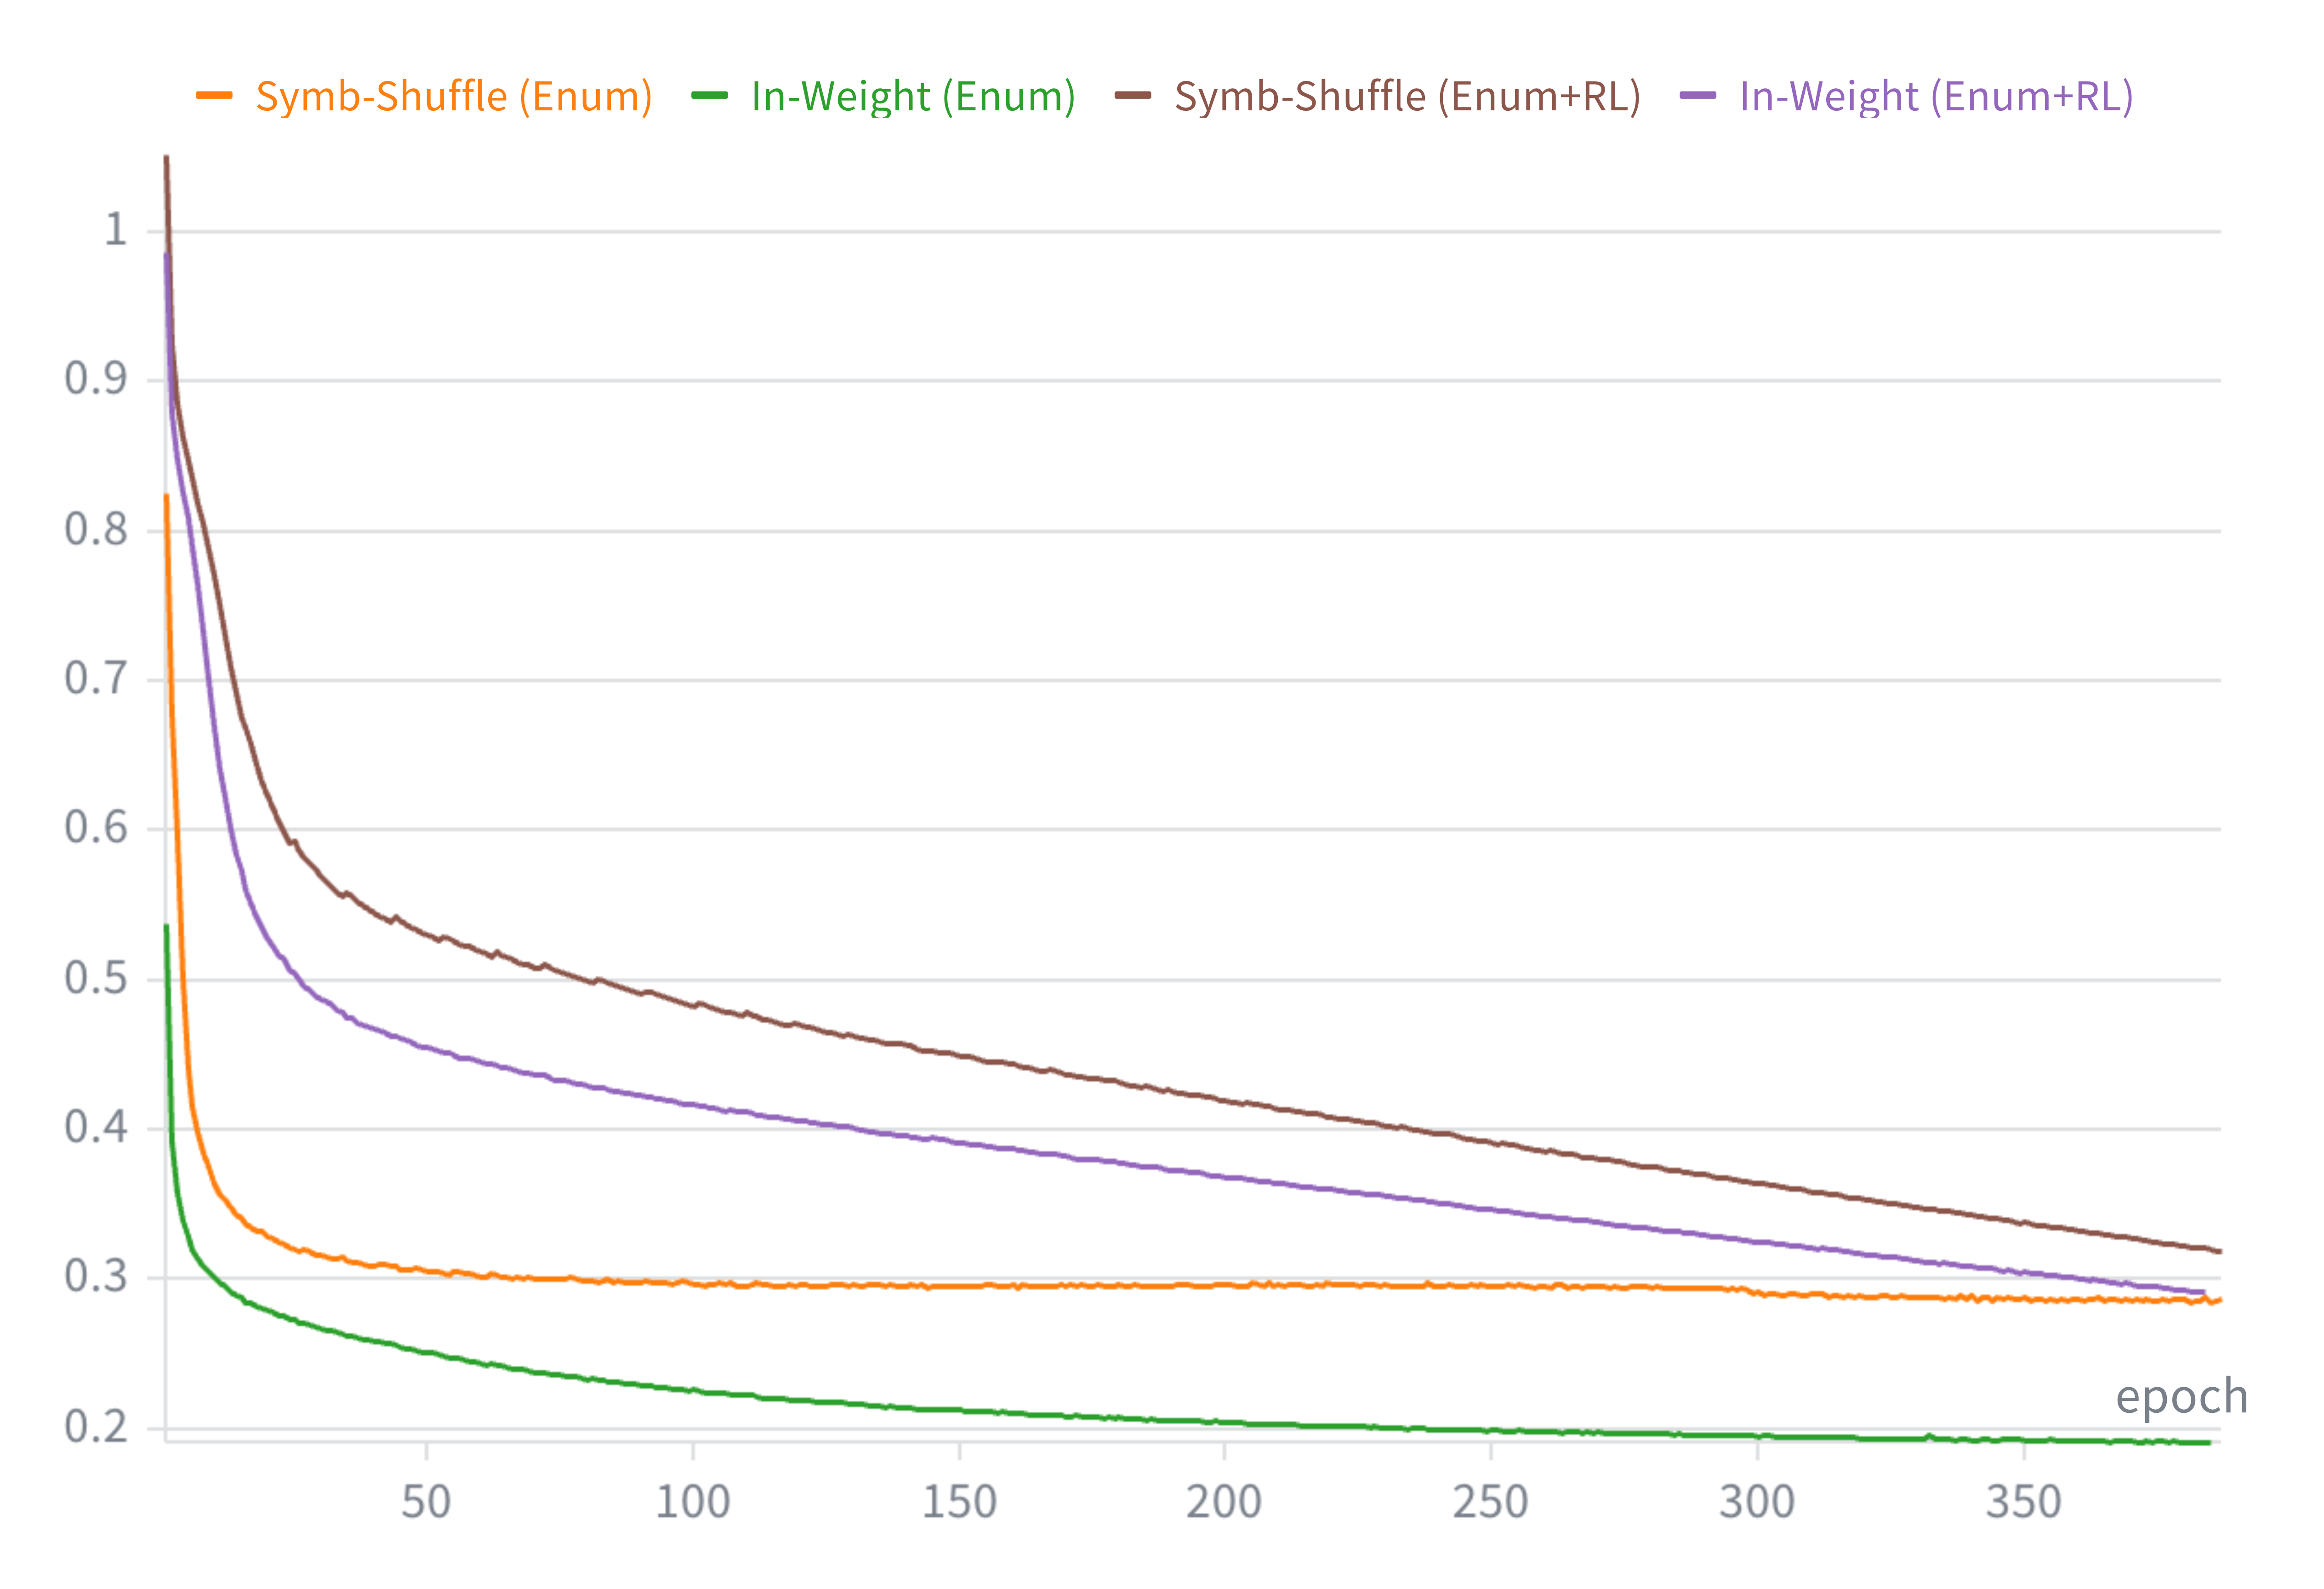
\includegraphics[width=\linewidth]{media/training/train_loss.png}
        \caption{Train loss}
        \label{fig:train-loss}
    \end{subfigure}\hfill
    \begin{subfigure}[t]{0.33\textwidth}
        \centering
        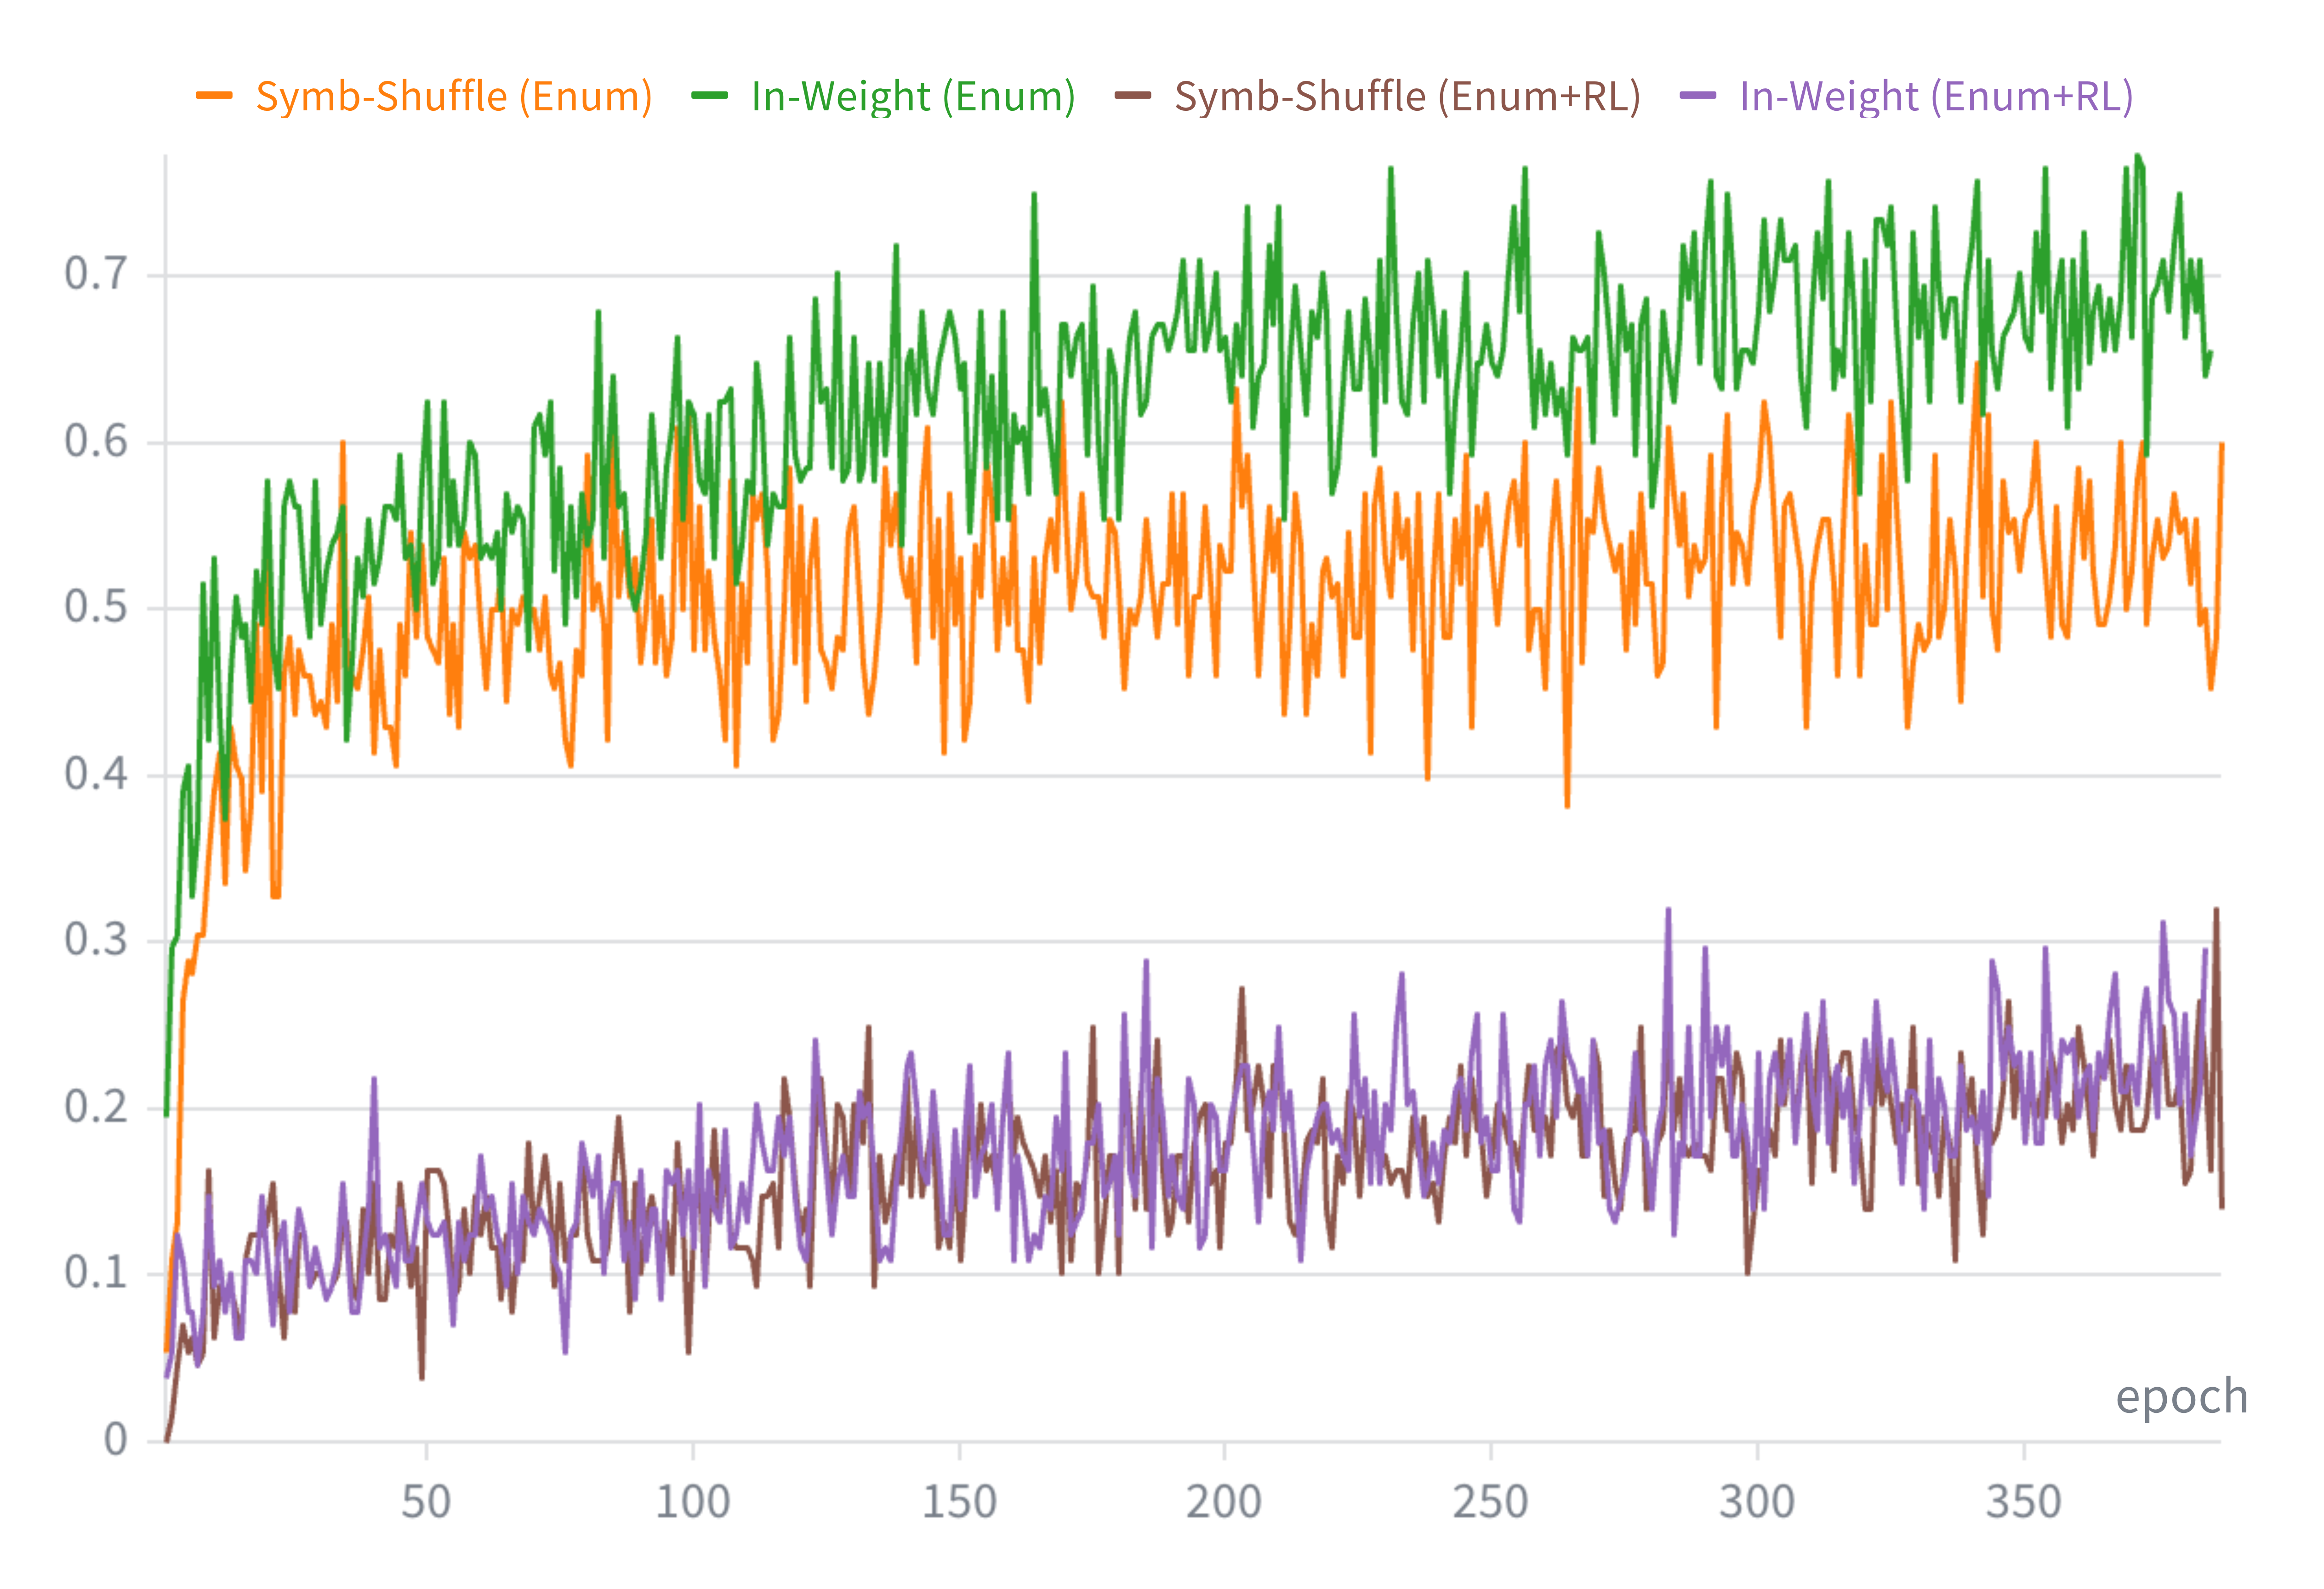
\includegraphics[width=\linewidth]{media/training/train_acc.png}
        \caption{Train accuracy}
        \label{fig:train-acc}
    \end{subfigure}\hfill
    \begin{subfigure}[t]{0.33\textwidth}
        \centering
        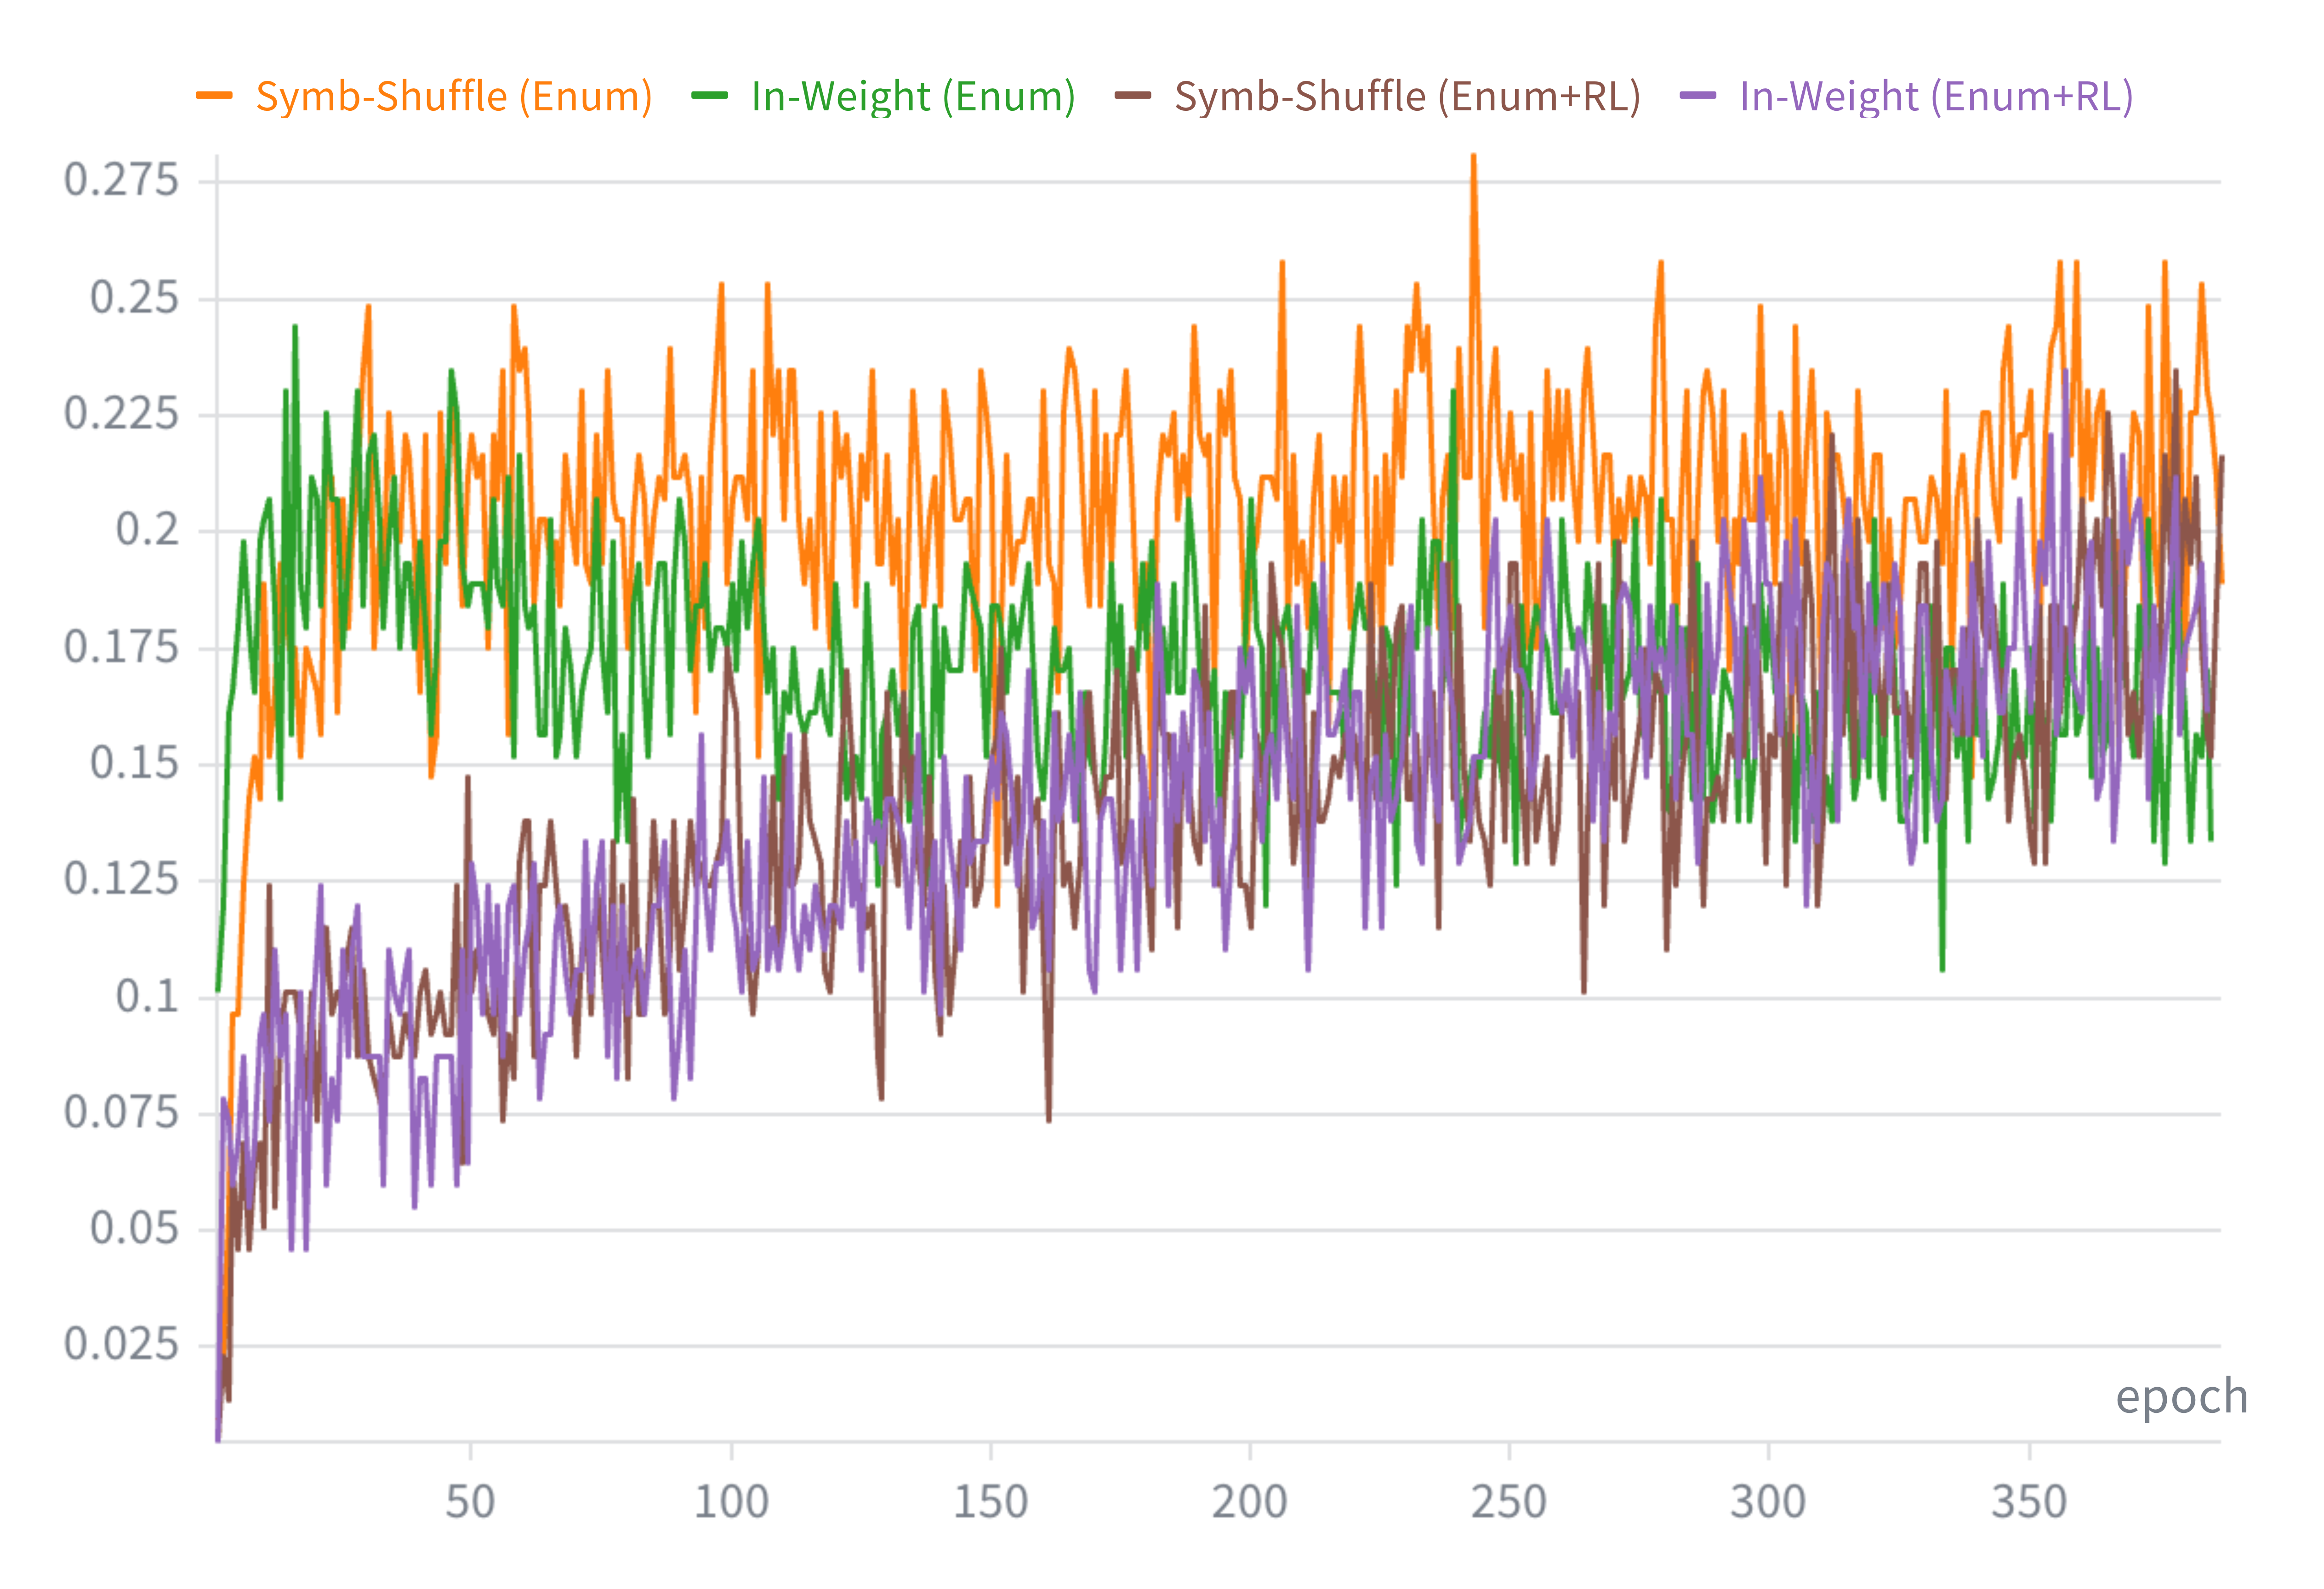
\includegraphics[width=\linewidth]{media/training/val_acc.png}
        \caption{Validation accuracy}
        \label{fig:val-acc}
    \end{subfigure}
    \caption{Training and validation cross-entropy loss and program induction accuracy for the four model variants over the full run. Per-task accuracy is 1 when the model's decoded program correctly maps all input examples to their corresponding outputs, and 0 otherwise.}
    \label{fig:training-curves}
\end{figure}

\Cref{fig:training-curves} compares the four model--corpus combinations across the full training run. Notably, on the smaller \textsc{Enum} corpus, the in-weight model achieves the lowest training loss and the highest training accuracy, but the symbol-shuffling variant matches or exceeds it on validation accuracy, hovering around $20$--$25\%$ against the in-weight model's $15$--$20\%$. This reflects the data-limited regime in which meta-learning is hypothesised to help: when each program is seen many times, the in-weight model overfits and memorises solutions, whereas symbol shuffling entails that no progra-permutation pair is seen more than once during training, forcing the meta-learning model to learn other generalising solutions. On the \textsc{Enum+RL} corpus the two models converge on validation accuracy (both around $15$--$20\%$), suggesting the dataset is large enough that the in-weight model cannot memorise solutions and is also forced to generalise.

\subsection{Probing}
\label{sec:results-probing}

\begin{figure}[t]
    \centering
    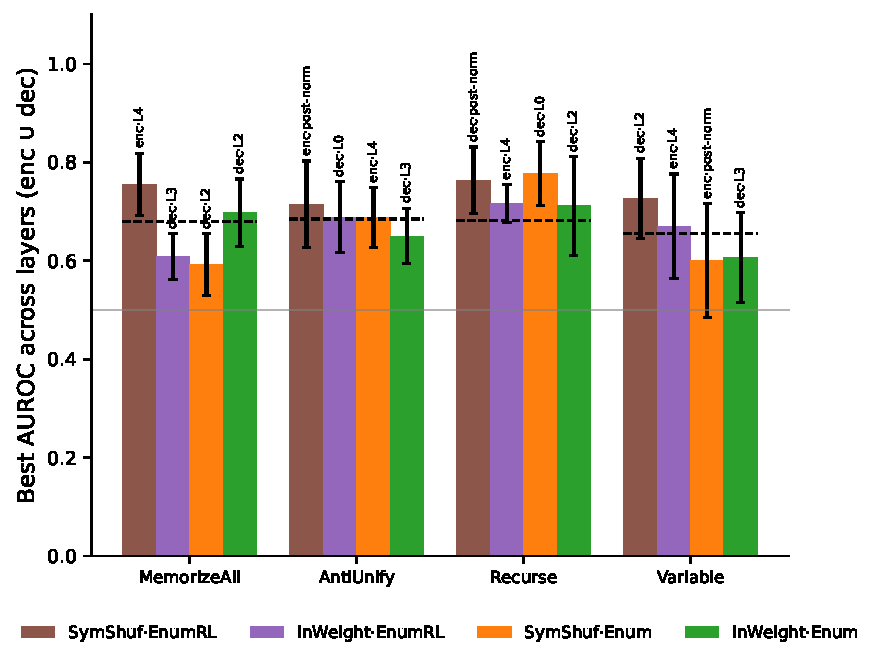
\includegraphics[width=0.78\textwidth]{media/probing/bars_max_per_primitive.pdf}
    \caption{Best AUROC across the layer sweep for each model on the four metaprimitives that are sufficiently represented in the $73$ MPL-acquired tasks. Bars are calculated w.r.t. the most predictive layer in each model with fold-level standard errors; the annotation above each bar is the layer with the winning representation. The dashed black segment in each group is the $95$th percentile of the label-shuffle null AUROC; the grey horizontal line marks AUROC $= 0.5$.}
    \label{fig:probing-bars}
\end{figure}

Only four of the seven metaprimitives in our vocabulary (\textsc{MemorizeAll}, \textsc{AntiUnify}, \textsc{Recurse}, \textsc{Variable}) were represented enough in MPL-acquired solutions to be valid probing targets; the probing results are seen in \Cref{fig:probing-bars}. Three patterns are visible:
\begin{enumerate}
    \item The symbol-shuffling model trained on \textsc{Enum+RL} achieves the highest AUROC on three of the four primitives (\textsc{MemorizeAll}, \textsc{Recurse}, \textsc{Variable}) and is closely tied for the highest on \textsc{AntiUnify}, where the other symbol-shuffling model trained on \textsc{Enum} achieves the highest AUROC. In every case, the symbol-shuffling model trained on \textsc{Enum+RL} achieves an AUROC at or above the corrected chance line. Meanwhile, its in-weight counterpart trained on the same corpus achieves a lower AUROC at every metaprimitive, suggesting that meta-learning via symbol-shuffling may be conducive towards a model developing metaprimitive-like representations, beyond the influence of generalisation pressure from a large dataset alone; for if a large dataset were sufficient, then the in-weight counterpart should demonstrate similarly high AUROC values.
    \item The meta-learning advantage partially transfers over to the smaller \textsc{Enum} corpus: the symbol-shuffling model trained on \textsc{Enum} matches the larger meta-learned model on \textsc{AntiUnify} and \textsc{Recurse}, despite seeing only the bottom-up portion of the corpus, and achieves higher or comparable AUROC to its in-weight counterpart on three out of the four metaprimitives.
    \item The layer of the winning representation is different across metaprimitives and models, and is found roughly evenly across the encoder and the decoder rather than concentrated in any one block. This suggests that metaprimitive-like representations, if they exist, are likely distributed across multiple layers in a Transformer's computation.
\end{enumerate}

However, there are also a few important caveats to be noted regarding the power and limitations of linear regression. A linear probe is a weak readout and does not account for primitives that are non-linearly encoded. We therefore interpret high AUROCs as positive evidence that the primitive is \emph{linearly} recoverable; low AUROCs do not guarantee that metaprimitives are not represented, but rather that they are not linearly recoverable. Conversely, a high AUROC means the embedding co-varies with the primitive label, but \emph{not} that the network actually computes with the primitive during inference \citep{belinkov2022probing}. Despite these caveats, a probing comparison across models is still valuable: holding the probe family and the training labels fixed, a systematic gap between symbol-shuffling and in-weight models is suggestive about whether meta-learning has reorganised model representations.

\subsection{Clustering and Error Similarity}
\label{sec:results-cluster-err}

\begin{figure}[t]
    \centering
    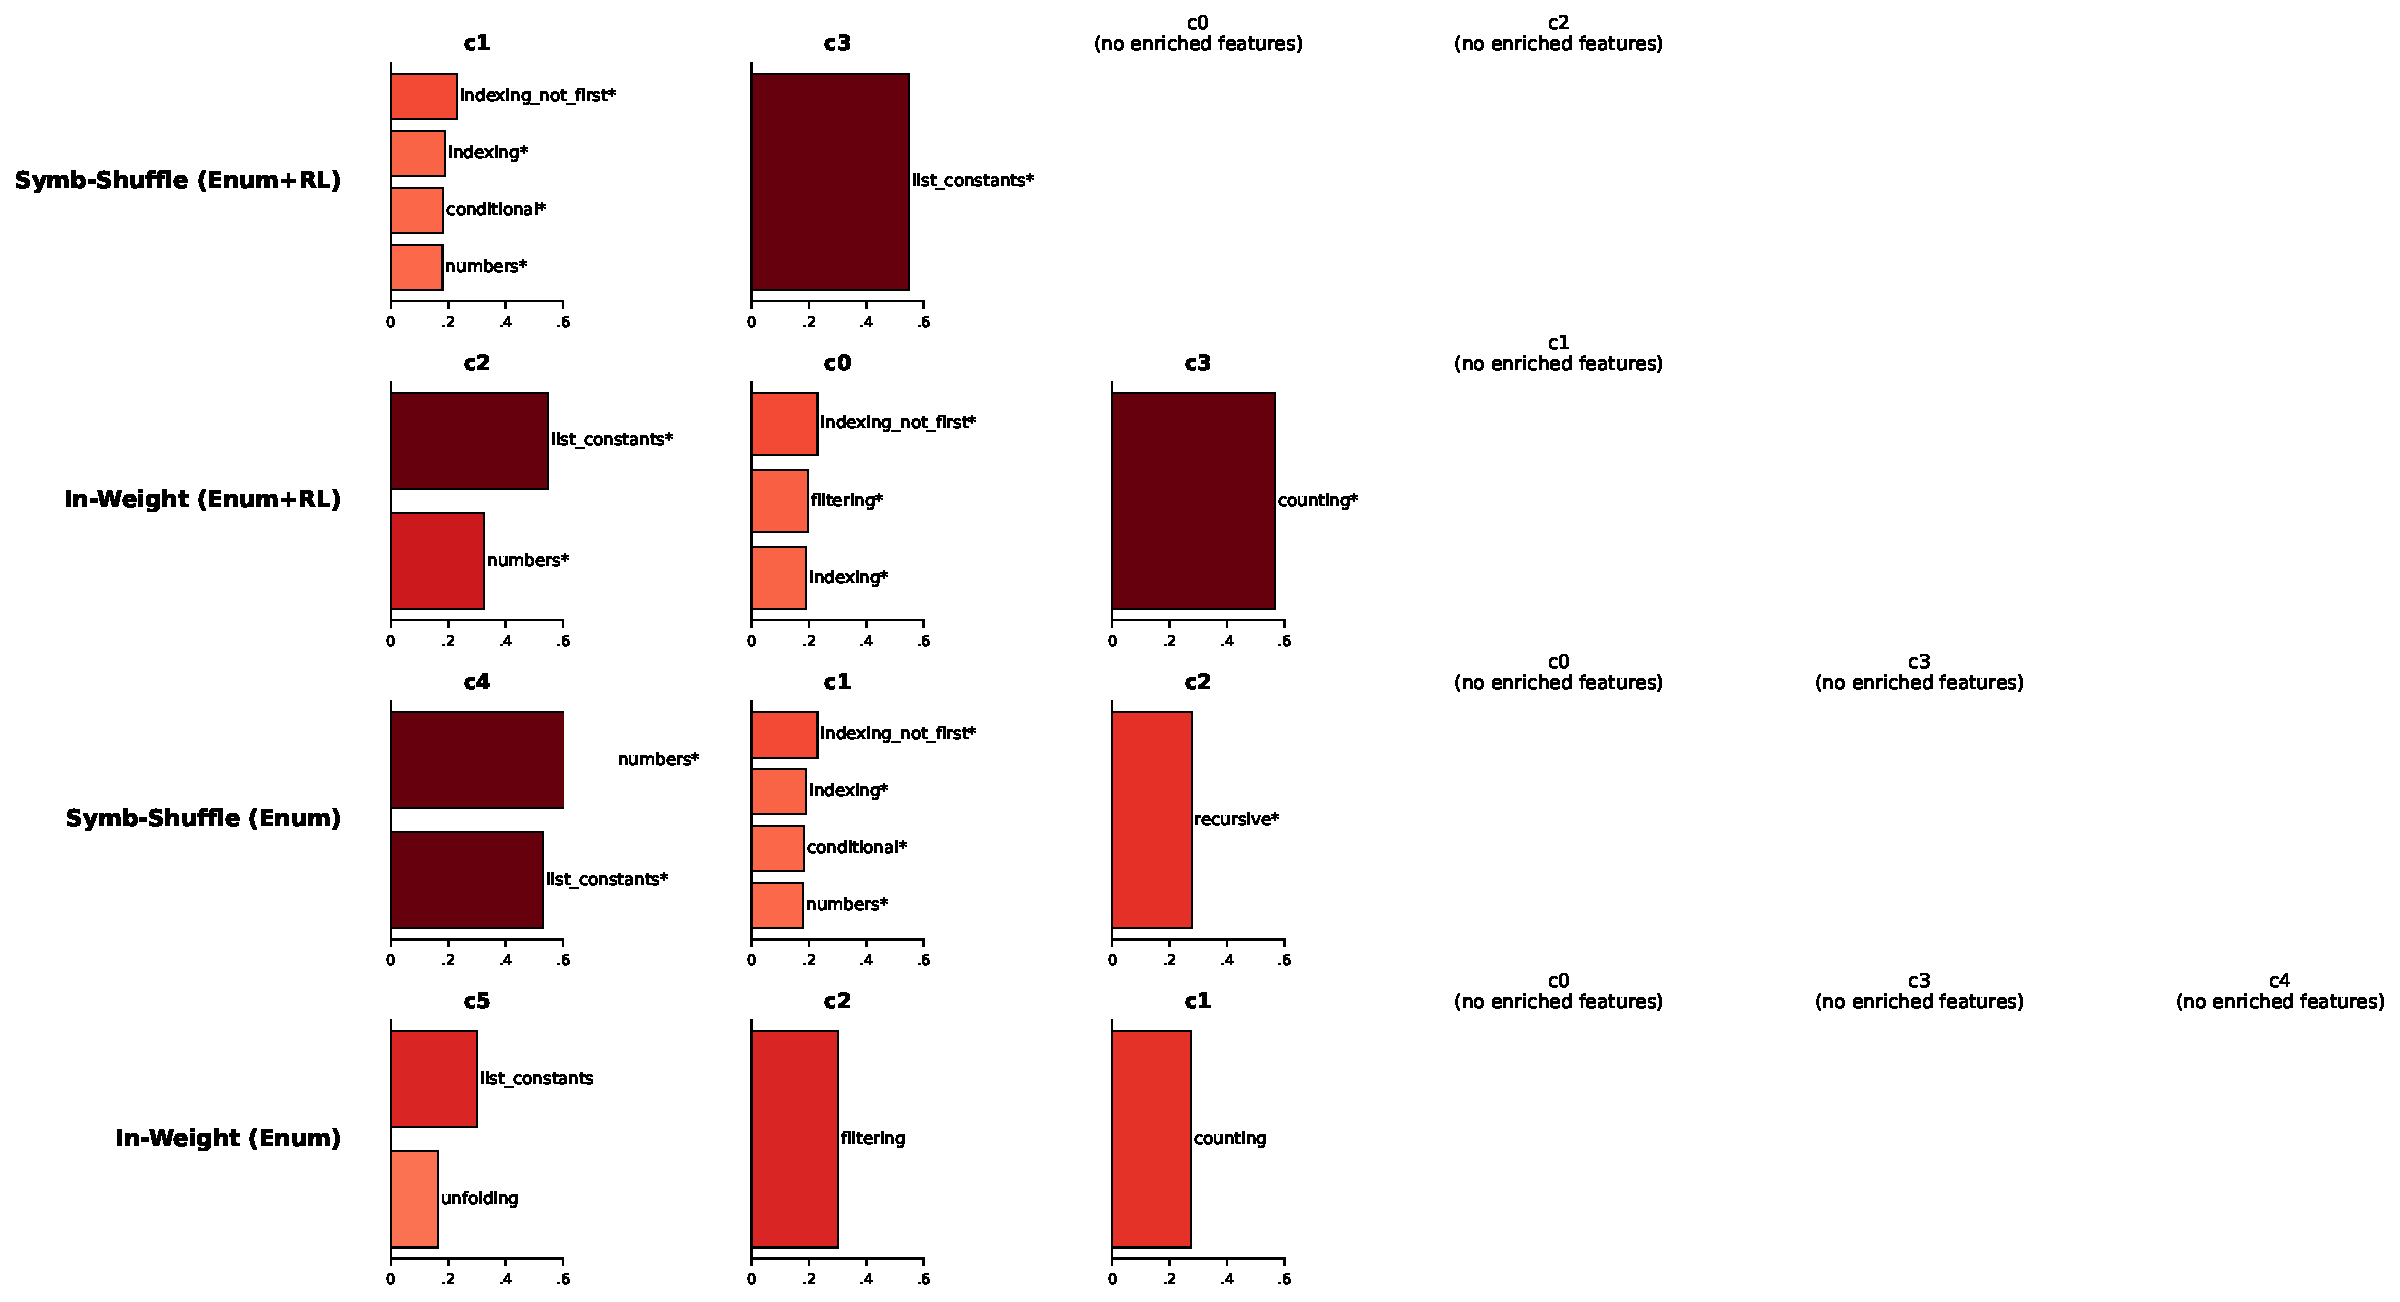
\includegraphics[width=0.9\textwidth]{media/clustering/cluster_portraits_cognitive_enriched.pdf}
    \caption{Top positively-enriched cognitive features per cluster for each model; see \Cref{tab:cognitive-tags} for a description of each feature as introduced by \citet{rule2024symbolic}. Bar length is the within-cluster enrichment of a feature (increase in probability of appearance inside a cluster vs overall validation set); an asterisk marks features that pass $\chi^2$ with Benjamini--Hochberg FDR at $q<0.05$. $k$ is selected by silhouette on the full embedding (\cref{app:analysis}).}
    \label{fig:clustering-portraits}
\end{figure}

\Cref{fig:clustering-portraits} shows the cognitive-feature signature, provided by \citet{rule2024symbolic}, of each $k$-means cluster on the per-task encoder output embeddings of the four models. Despite training on different corpora, a \texttt{list\_constants/numbers} cluster recurs across all models, grouping tasks whose solutions depend on list construction with specific integer constants. Moreover, both symbol-shuffling methods spontaneously learn an identical cluster with \texttt{indexing\_not\_first}, \texttt{indexing}, \texttt{conditional}, and \texttt{numbers} features, suggesting that meta-learning encourages grouping of tasks at the primitive level based on conditional access of particular list indices. However, there is a similar cluster of \texttt{indexing\_not\_first}, \texttt{indexing}, and \texttt{filtering} features for the in-weight model trained on the \textsc{Enum+RL} dataset, so it seems that this cluster is not unique to meta-learners, but may be broadly useful across many models.

\begin{figure}[t]
    \centering
    \begin{subfigure}[t]{0.45\textwidth}
        \centering
        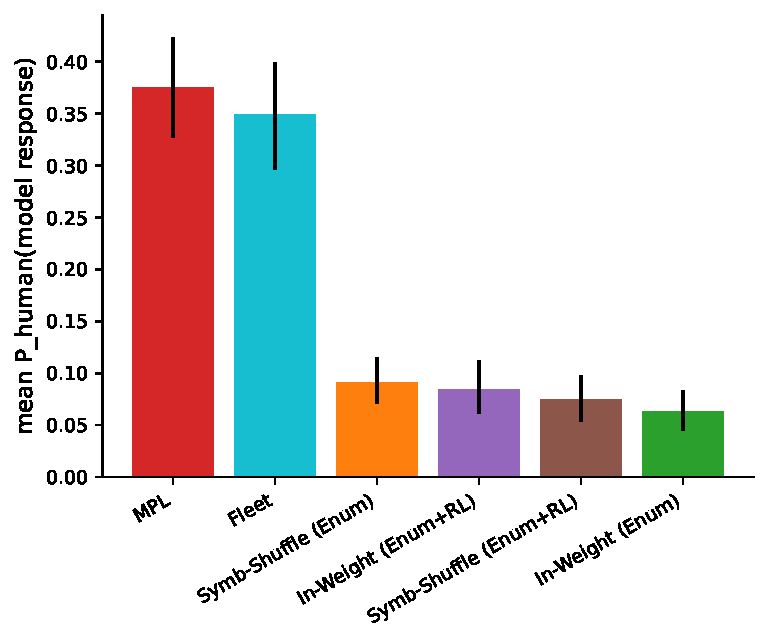
\includegraphics[width=\linewidth]{media/error_similarity/bar_human_likeness.pdf}
        \caption{Mean human-likeness across all validation tasks from \citet{rule2024symbolic}.}
        \label{fig:err-marginal}
    \end{subfigure}\hfill
    \begin{subfigure}[t]{0.45\textwidth}
        \centering
        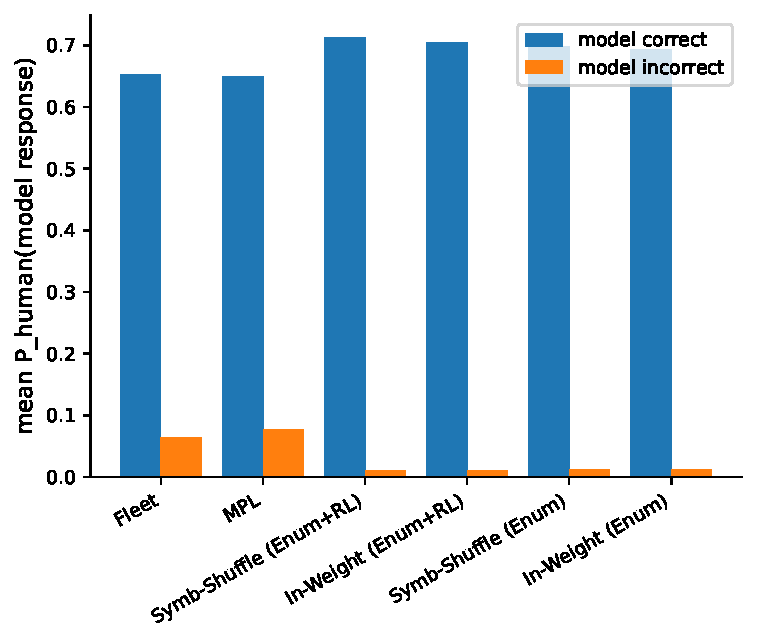
\includegraphics[width=\linewidth]{media/error_similarity/bars_conditional.pdf}
        \caption{Mean human-likeness conditioned on model correctness.}
        \label{fig:err-conditional}
    \end{subfigure}
    \caption{Per-method mean human-likeness $\mathbb{E}\bigl[P_{\mathrm{human}}(r_{\mathrm{model}})\bigr]$ over the 100 validation tasks from \citet{rule2024symbolic}. The conditional panel splits each method's mean into cells where the model produced the gold response and cells where it did not (right).}
    \label{fig:err-bars}
\end{figure}

The error-similarity analysis (\cref{fig:err-bars}) demonstrate the limitations of our models in approximating human behaviour, despite potential representational alignments to the human-like MPL algorithm of \citet{rule2024symbolic}. All four Transformers sit between $6-10\%$ mean human-likeness in their outputs, an order of magnitude below MPL ($\approx 38\%$) and Fleet ($\approx 35\%$). Moreover, when Transformers fail to solve a task, their errors are characteristically non-human, in contrast to MPL and Fleet whose failure modes themselves overlap with human errors. Note that the high human-likeness on correct outputs is not a very informative measure: it reflects Transformers succeeding on easy tasks without a lot of human disagreement, but does not tell us about their error modes.

\section{Conclusion}
\label{sec:conclusion}

We introduce a symbol-shuffling framework to train meta-learning models on program induction, utilising list manipulation tasks similar to those in \citet{rule2024symbolic}. We compare symbol-shuffling models with their in-weight counterparts to demonstrate that meta-learning may increase representational alignment of models with metaprimitive-based search algorithms, but does not necessarily make them more human-like in their outputs or errors. In the creation of this dataset, we also took inspiration from the programming language literature to develop a framework for synthesising a large number of high-quality program induction examples from a set of well-typed primitives, employing bottom-up enumeration with filtering followed by reinforcement learning for program generation.

The probing methods used to analyse model representations is limited in its robustness to non-linear relationships, and more importantly, does not provide mechanistic evidence for the existence or manipulation of metaprimitives within models. A mechanistic account of metaprimitive use in meta-learning models or a plausible account of its emergence during training, together with improving model validation accuracy to human levels, are crucial next steps for extending this work and its impact.

\bibliographystyle{plainnat}
\bibliography{references}

\newpage

\appendix

\section{Declaration of Generative AI Usage}
\label{app:llm}

Large Language Model (LLM) services including Claude and ChatGPT were used to help in the preparation of this paper, including:\begin{itemize}
    \item Conducting literature review and explaining papers, methods, and results.
    \item Drafting portions of the paper (particularly the appendices), subsequently subject to human review and editing.
    \item Drafting portions of the code used to run the experiments and visualise results, subsequently subject to human review and editing.
\end{itemize}

\section{Code and Data Availability}
\label{app:code-data}

The code used to generate the dataset, train the models, and run the analyses is available at the following GitHub repository: \href{https://github.com/PerceptronV/mlmp}{https://github.com/PerceptronV/mlmp}.

\section{DSL Specification}
\label{app:dsl-specification}

We adopt the typed lambda-calculus DSL of \citet{rule2024symbolic}, used in both their Metaprogram Learner (MPL) and the human 100-task list-function benchmark from which our task pool is drawn. The DSL is a simply-typed lambda calculus extended with conditionals and a fixed set of 57 primitive functions over the type universe $\{\texttt{Int}, \texttt{Bool}, \texttt{[Int]}, \texttt{[Bool]}, \texttt{[[Int]]}\}$. Programs are S-expressions; for example, the program that drops the last element of a list and reverses what remains is written \texttt{(reverse (droplast 1 x))}.

\subsection{Built-in expressions}

The expression language is
\[
  e \;::=\; c \;\mid\; x \;\mid\; (f\;e_1\;\cdots\;e_k)
         \;\mid\; (\lambda\;(x_1\;\cdots\;x_k)\;e)
         \;\mid\; (\mathrm{if}\;e_1\;e_2\;e_3),
\]
where $c$ ranges over integer, boolean, and empty-list literals, $x$ over variables, and $f$ over primitive function symbols. The base types are $\texttt{Int}$ and $\texttt{Bool}$; list types $[\sigma]$ and function types $\sigma \to \tau$ are formed inductively. Type variables on the polymorphic primitives are instantiated to types within the universe above. All synthesised top-level programs have type $[\texttt{Int}] \to [\texttt{Int}]$.

\subsection{Primitive functions}

\Cref{tab:dsl-primitives} reproduces the primitive set, types, and informal descriptions, identical to the DSL of \citet{rule2024symbolic}.

\begin{table}[!htbp]
\centering
\caption{Primitive functions in the DSL of \citep{rule2024symbolic}. Polymorphic type variables are written in terms of type variables \texttt{t1}, \texttt{t2}.}
\label{tab:dsl-primitives}
\tiny
\begin{tabular}{lll}
\toprule
Usage & Type & Description \\
\midrule
\multicolumn{3}{l}{\textit{Lambda, literals, control flow}} \\
$(\lambda\;x\;\mathit{body})$           & \texttt{t1 -> t2 -> (t1 -> t2)}   & lambda abstraction; binds $x$ in $\mathit{body}$ \\
$0, 1, 2, \ldots, 99$                   & \texttt{Int}                       & natural numbers \\
\texttt{true, false}                    & \texttt{Bool}                      & Boolean values \\
$[\,]$                                  & \texttt{[t1]}                      & empty list \\
$(\mathrm{if}\;p\;a\;b)$                & \texttt{Bool -> t1 -> t1 -> t1}   & $a$ if $p$ is true, else $b$ \\
$(==\;x\;y)$                            & \texttt{t1 -> t1 -> Bool}         & true if $x$ and $y$ are structurally identical \\
\midrule
\multicolumn{3}{l}{\textit{Arithmetic and predicates}} \\
$(+\;x\;y),\ (-\;x\;y),\ (*\;x\;y)$     & \texttt{Int -> Int -> Int}        & add, subtract, multiply \\
$(/\;x\;y),\ (\%\;x\;y)$                & \texttt{Int -> Int -> Int}        & quotient, remainder \\
$(<\;x\;y),\ (>\;x\;y)$                 & \texttt{Int -> Int -> Bool}       & strict comparison \\
$(\texttt{is\_even}\;x),\ (\texttt{is\_odd}\;x)$ & \texttt{Int -> Bool}      & parity \\
$(\texttt{and}\;x\;y),\ (\texttt{or}\;x\;y)$ & \texttt{Bool -> Bool -> Bool} & Boolean conjunction, disjunction \\
$(\texttt{not}\;x)$                     & \texttt{Bool -> Bool}             & Boolean negation \\
\midrule
\multicolumn{3}{l}{\textit{List construction, indexing}} \\
$(\texttt{singleton}\;x)$               & \texttt{t1 -> [t1]}               & single-element list \\
$(\texttt{repeat}\;x\;n)$               & \texttt{t1 -> Int -> [t1]}        & list repeating $x$, $n$ times \\
$(\texttt{range}\;i\;j\;n)$             & \texttt{Int -> Int -> Int -> [Int]} & inclusive range from $i$ to $j$ by $n$ \\
$(\texttt{cons}\;x\;\mathit{xs})$       & \texttt{t1 -> [t1] -> [t1]}       & prepend $x$ to $\mathit{xs}$ \\
$(\texttt{append}\;\mathit{xs}\;x)$     & \texttt{[t1] -> t1 -> [t1]}       & append $x$ to $\mathit{xs}$ \\
$(\texttt{concat}\;\mathit{xs}\;\mathit{ys})$ & \texttt{[t1] -> [t1] -> [t1]} & concatenation \\
$(\texttt{first}/\texttt{second}/\texttt{third}/\texttt{last}\;\mathit{xs})$
                                        & \texttt{[t1] -> t1}               & positional access \\
$(\texttt{nth}\;i\;\mathit{xs})$        & \texttt{Int -> [t1] -> t1}        & element at index $i$ \\
\midrule
\multicolumn{3}{l}{\textit{List manipulation}} \\
$(\texttt{insert}\;x\;i\;\mathit{xs})$  & \texttt{t1 -> Int -> [t1] -> [t1]} & insert at index $i$ \\
$(\texttt{replace}\;i\;x\;\mathit{xs})$ & \texttt{Int -> t1 -> [t1] -> [t1]} & replace at $i$ \\
$(\texttt{swap}\;i\;j\;\mathit{xs})$    & \texttt{Int -> Int -> [t1] -> [t1]} & swap indices $i,j$ \\
$(\texttt{cut\_idx}\;i\;\mathit{xs})$   & \texttt{Int -> [t1] -> [t1]}      & remove at index $i$ \\
$(\texttt{cut\_val}\;x\;\mathit{xs})$   & \texttt{t1 -> [t1] -> [t1]}       & remove first occurrence of $x$ \\
$(\texttt{cut\_vals}\;x\;\mathit{xs})$  & \texttt{t1 -> [t1] -> [t1]}       & remove all occurrences of $x$ \\
$(\texttt{drop}\;n\;\mathit{xs})$       & \texttt{Int -> [t1] -> [t1]}      & drop first $n$ \\
$(\texttt{droplast}\;n\;\mathit{xs})$   & \texttt{Int -> [t1] -> [t1]}      & drop last $n$ \\
$(\texttt{cut\_slice}\;i\;j\;\mathit{xs})$ & \texttt{Int -> Int -> [t1] -> [t1]} & remove elements at indices $i$ to $j$ inclusive \\
$(\texttt{take}\;n\;\mathit{xs})$       & \texttt{Int -> [t1] -> [t1]}      & first $n$ elements \\
$(\texttt{takelast}\;n\;\mathit{xs})$   & \texttt{Int -> [t1] -> [t1]}      & last $n$ elements \\
$(\texttt{slice}\;i\;j\;\mathit{xs})$   & \texttt{Int -> Int -> [t1] -> [t1]} & sublist from $i$ to $j$ inclusive \\
$(\texttt{splice}\;\mathit{ys}\;i\;\mathit{xs})$
                                        & \texttt{[t1] -> Int -> [t1] -> [t1]} & insert $\mathit{ys}$ into $\mathit{xs}$ at $i$ \\
$(\texttt{zip}\;\mathit{xs}\;\mathit{ys})$ & \texttt{[t1] -> [t1] -> [[t1]]} & pairs $\mathit{xs}$ and $\mathit{ys}$ pointwise \\
$(\texttt{is\_in}\;\mathit{xs}\;x)$     & \texttt{[t1] -> t1 -> Bool}       & membership test \\
\midrule
\multicolumn{3}{l}{\textit{Aggregation and structural}} \\
$(\texttt{length}\;\mathit{xs})$        & \texttt{[t1] -> Int}              & length \\
$(\texttt{max}\;\mathit{xs})$           & \texttt{[Int] -> Int}             & maximum \\
$(\texttt{min}\;\mathit{xs})$           & \texttt{[Int] -> Int}             & minimum \\
$(\texttt{product}\;\mathit{xs})$       & \texttt{[Int] -> Int}             & product of elements \\
$(\texttt{sum}\;\mathit{xs})$           & \texttt{[Int] -> Int}             & sum of elements \\
$(\texttt{unique}\;\mathit{xs})$        & \texttt{[t1] -> [t1]}             & unique elements \\
$(\texttt{reverse}\;\mathit{xs})$       & \texttt{[t1] -> [t1]}             & reversal \\
$(\texttt{flatten}\;\mathit{xs})$       & \texttt{[[t1]] -> [t1]}           & concatenate list of lists \\
\midrule
\multicolumn{3}{l}{\textit{Higher-order}} \\
$(\texttt{map}\;f\;\mathit{xs})$        & \texttt{(t1 -> t2) -> [t1] -> [t2]}    & apply $f$ to each element \\
$(\texttt{mapi}\;f\;\mathit{xs})$       & \texttt{(Int -> t1 -> t2) -> [t1] -> [t2]} & like \texttt{map}, with index \\
$(\texttt{filter}\;p\;\mathit{xs})$     & \texttt{(t1 -> Bool) -> [t1] -> [t1]}      & keep elements where $p$ is true \\
$(\texttt{filteri}\;p\;\mathit{xs})$    & \texttt{(Int -> t1 -> Bool) -> [t1] -> [t1]} & like \texttt{filter}, with index \\
$(\texttt{fold}\;f\;\mathit{acc}\;\mathit{xs})$
                                        & \texttt{(t2 -> t1 -> t2) -> t2 -> [t1] -> t2} & iterative accumulation \\
$(\texttt{foldi}\;f\;\mathit{acc}\;\mathit{xs})$
                                        & \texttt{(Int -> t2 -> t1 -> t2) -> t2 -> [t1] -> t2} & like \texttt{fold}, with index \\
$(\texttt{count}\;x\;\mathit{xs})$      & \texttt{(t1 -> Bool) -> [t1] -> Int} & count elements satisfying predicate \\
$(\texttt{find}\;p\;\mathit{xs})$       & \texttt{(t1 -> Bool) -> [t1] -> [Int]} & indices where $p$ is true \\
$(\texttt{sort}\;f\;\mathit{xs})$       & \texttt{(t1 -> Int) -> [t1] -> [t1]} & sort by key \\
$(\texttt{group}\;f\;\mathit{xs})$      & \texttt{(t1 -> t2) -> [t1] -> [[t1]]} & group by key \\
\bottomrule
\end{tabular}
\end{table}

\subsection{Semantics and runtime guards}

The evaluator in our code implements call-by-value semantics on the AST. Several operations carry runtime guards: integer division and modulo by zero raise an error and are recorded as crashes ($\dagger$) in the fingerprint; positional accessors (\texttt{first}, \texttt{nth}, \texttt{max}, etc.) error on lists too short to be served, and \texttt{insert}/\texttt{replace}/\texttt{swap}/\texttt{cut\_idx} error on out-of-bounds indices. List-producing primitives are gated by a hard cap of $\texttt{MAX\_LIST\_SIZE} = 1000$ to prevent expressions such as \texttt{(repeat $x$ $n$)} with adversarial $n$ from exhausting memory; over-cap evaluations are also recorded as crashes. Following \citet{rule2024symbolic}, integer literals are drawn from $\{0,\ldots,99\}$ in the program-induction tasks.

\subsection{Differences from \citet{rule2024symbolic}}

The primitive set, type universe, and S-expression surface syntax are identical to those used in MPL. Two implementation-level details differ. First, \texttt{range} in our implementation produces an \emph{inclusive} range from $i$ to $j$ by $n$ (matching the description in \citet{rule2024symbolic}'s table). Second, our enumerator and RL learner expose integer literals as holes $\square_{\mathbb{Z}}$ rather than as named constants, with concrete instantiations sampled from the seed set $C_{\mathrm{seed}} = \{0, 1, \ldots, 10\}$ at corpus-expansion time (\cref{app:enumeration-rl}); this differs from MPL, which samples integer literals directly within MCMC.

\section{Combining Bottom-Up Enumeration and Reinforcement Learning for Program Synthesis}
\label{app:enumeration-rl}

This appendix gives the algorithmic and parametric detail needed to reproduce the enumeration and RL phases of \cref{sec:dataset-generation}. 

\subsection{Problem setting}\label{app:enum-rl-problem}

Given (i) the typed lambda-calculus DSL of \cref{app:dsl-specification}, where every primitive is black-box callable but not necessarily described in closed form, and (ii) a reward function $R$ mapping a program to a real value, we want to synthesise a large set of programs that are pairwise behaviourally distinct and individually achieve high reward (with $R$ chosen here to reward output variability and behavioural novelty). The pipeline has two phases:
\begin{enumerate}
  \item \textbf{Bottom-up enumeration} of all programs up to a size cap $s_{\max}$, deduplicated by behaviour on a fixed test suite (\cref{app:enum}).
  \item \textbf{Priority-queue reinforcement learning} \citep{abolafia2018priority} that warm-starts on the enumerated corpus and then extends it to larger programs via on-policy sampling against a top-$K$ buffer (\cref{app:rl}).
\end{enumerate}
Programs are stored as \emph{sketches}: ASTs in which every integer literal position is replaced by a placeholder $\square_{\mathbb{Z}}$. A sketch becomes a concrete program under a \emph{substitution} $\sigma$, an integer list indexing the holes in pre-order.

\subsection{Part I: Bottom-up enumeration}\label{app:enum}

\paragraph{Size metric.} Every AST node carries an integer size, defined inductively:

\begin{center}
\begin{tabular}{ll}
\toprule
Node & Size \\
\midrule
Literal, variable, empty list, hole $\square_{\mathbb{Z}}$ & $1$ \\
Application $(f\;a_1\;\cdots\;a_k)$ & $1 + |a_1| + \cdots + |a_k|$ \\
Lambda $(\lambda\;(p_1\;\cdots\;p_k)\;e)$ & $1 + |e|$ \\
Conditional $(\mathrm{if}\;c\;t\;e)$ & $1 + |c| + |t| + |e|$ \\
\bottomrule
\end{tabular}
\end{center}

The size of the function symbol in an application is subsumed into the application node's unit cost. Enumeration proceeds by increasing size: programs of size $s$ are built exclusively from sub-expressions of size $<s$.

\paragraph{Observational equivalence.} Fix a test suite $T = \{t_1, \ldots, t_m\}$ of $m$ inputs ($m = 10$, listed below). The \emph{fingerprint} of a closed program $p:\tau \to \upsilon$ is
\[
  \Phi(p) \;=\; \bigl(p(t_1), \ldots, p(t_m)\bigr) \in (\upsilon \cup \{\dagger\})^m,
\]
where $\dagger$ marks a failed evaluation (runtime or type error, or list-size cap violation). Two programs of the same type are observationally equivalent if their fingerprints are equal. The default test suite is
\[
  T = \{[], [0], [3,1,2], [1,1,1,1], [5,4,3,2,1], [1,2,3,4,5,6,7,8],
\]
\[
  [10,-3,7,7,0], [2,8,3,8,2,3], [0,1,0,1,0], [42]\},
\]
chosen by hand to span empty, singleton, sorted, reverse-sorted, duplicate-heavy, binary, negative-containing, and long inputs.

\paragraph{Open terms.} Higher-order primitives demand candidate \emph{open} terms (lambda bodies) with free variables beyond the top-level input $x$. For an open term $e$ with free variables $y_1: \sigma_1, \ldots, y_k: \sigma_k$ (in addition to $x$), the fingerprint is computed over the Cartesian product $T \times V_1 \times \cdots \times V_k$ where each $V_i$ is a small probe set for type $\sigma_i$:
\[
  V_{\texttt{Int}} = \{0,1,3\}, \quad V_{\texttt{Bool}} = \{\top,\bot\}, \quad V_{\texttt{[Int]}} = \{[], [1], [2,1,3]\}, \quad V_{\texttt{[Bool]}} = \{[], [\top], [\top,\bot]\},
\]
where $\top, \bot$ are the boolean literals for true and false, respectively.
Two open terms are equivalent iff they agree on this full probe grid.

\paragraph{Integer holes and the probe sequence.} Instead of seeding many integer literal variants, the base case includes a single hole $\square_{\mathbb{Z}}:\texttt{Int}$. To compute the fingerprint of a sketch $\pi$ with $k$ holes, the compiler substitutes the $i$-th hole (in pre-order) with $\mathrm{PROBE}[i \bmod |\mathrm{PROBE}|]$ where
\[
  \mathrm{PROBE} = [5, 3, 7, 2, 9, 0, 8, 1, 6, 4].
\]
The resulting fingerprint has the same arity as that of a concrete program. Two sketches that agree under this probe substitution are considered behaviourally equivalent; the false-equivalence rate is negligible in practice given the diversity of $T$. At expansion time, a sketch with $k$ holes is concretised by sampling $\sigma \in C_{\mathrm{seed}}^k$ with $C_{\mathrm{seed}} = \{0,\ldots,10\}$ (or enumerating $C_{\mathrm{seed}}^k$ exhaustively when small).

\paragraph{The program bank.} The bank $\mathcal{B}$ stores, for each $(\tau, s)$, one representative per observational equivalence class:
\[
  \mathcal{B}[\tau][s] = \bigl\{[p]_\sim \;\big|\; \vdash p : \tau,\; |p| = s\bigr\}.
\]
The bank is seeded at $s = 1$ with the hole $\square_{\mathbb{Z}}$, the boolean literals $\top, \bot$, empty lists $[\,]_\sigma$ for each list type $\sigma$, and the input variable $x:[\texttt{Int}]$.

\paragraph{First-order applications.} For a first-order primitive $f:A_1 \times \cdots \times A_k \to R$ and target size $s$, sub-expression sizes must satisfy $\sum_i s_i = s-1$ with $s_i \geq 1$. The enumerator forms
\[
  \mathcal{B}[R][s] \mathrel{+}= \bigl\{ (f\;a_1\;\cdots\;a_k) \;\big|\; a_i \in \mathcal{B}[A_i][s_i] \bigr\} / \!\sim.
\]
Polymorphic primitives are pre-expanded into all valid monomorphic instantiations over the concrete type universe.

\paragraph{Higher-order applications and nested lambdas.} When an argument position demands a function type $A_1 \times \cdots \times A_k \to B$, the lambda argument is synthesised inline. Given a size budget $b$ for the lambda, the typing context is extended by $\Gamma' = \Gamma \cup \{y_i:A_i\}$ and a child bank $\mathcal{B}'$ is enumerated over $\Gamma'$ up to size $b - 1$. Lambda candidates are then $\{(\lambda\;(y_1\;\cdots\;y_k)\;e) \;|\; e \in \mathcal{B}'[B][b-1]\}$. Child banks are cached by $(\Gamma', b)$. Lambda nesting is capped at $\ell_{\max} = 2$ to bound combinatorial blow-up while still admitting up to three-level nested lambdas inside higher-order arguments.

\paragraph{Quality filter.} Let $\mathcal{F}(p) \subseteq \{1,\ldots,m\}$ be the indices on which $p$ does not crash, and let $\mathrm{var}(p) = |\{p(t_i)\}_{i\in \mathcal{F}(p)}| / |\mathcal{F}(p)|$. A program is retained in the quality corpus iff (i) $|\mathcal{F}(p)| \geq 3$, (ii) $|\{p(t_i)\}_{i\in \mathcal{F}(p)}| \geq 2$, and (iii) $\mathrm{var}(p) \geq \nu_{\min} = 0.3$. The full bank (with and without quality filtering) is retained: the quality corpus drives warm-start training, the full bank drives sketch expansion.

\paragraph{Parameters used in the reported runs.}

\begin{center}
\small
\begin{tabular}{lll}
\toprule
Symbol & Value & Role \\
\midrule
$s_{\max}$       & $8$        & maximum AST size enumerated \\
$\ell_{\max}$    & $2$        & maximum lambda nesting depth in higher-order arguments \\
$\nu_{\min}$     & $0.3$      & minimum output variability \\
$|T|$            & $10$       & test-suite size for fingerprinting \\
$C_{\mathrm{seed}}$ & $\{0,\ldots,10\}$ & integer constants used for sketch expansion \\
PROBE            & $[5,3,7,2,9,0,8,1,6,4]$ & cyclic hole-probe sequence \\
\bottomrule
\end{tabular}
\end{center}

\paragraph{Sketch expansion.} After enumeration, every sketch in $\mathcal{B}$ is concretised by sampling substitutions $\sigma \sim \mathrm{Unif}(C_{\mathrm{seed}}^k)$ (or enumerating $C_{\mathrm{seed}}^k$ exhaustively when $|C_{\mathrm{seed}}|^k \leq N_{\mathrm{sub}}$). The per-sketch budget is derived from a global target $N_{\mathrm{target}} = 6{,}000{,}000$ as
\[
  N_{\mathrm{sub}} = \lceil N_{\mathrm{target}} / |\mathcal{B}|\rceil.
\]
Each concrete program is fingerprinted and admitted only if (i) it passes the quality filter and (ii) its fingerprint has not been seen before. The running fingerprint table is denoted \texttt{corpus\_fingerprints}.

\subsection{Part II: Reinforcement learning}\label{app:rl}

The RL phase trains a neural policy to generate programs top-down as a sequence of grammar-constrained AST-node choices. The MDP and training loop follow \citet{abolafia2018priority}, with three changes: (i) the action space is shaped by typing constraints rather than by a flat vocabulary, (ii) policies emit \emph{sketches} that are concretised after sampling, and (iii) the warm-start signal is the bottom-up enumeration corpus of \cref{app:enum}.

\paragraph{MDP state.} A synthesis state is a tuple $s = (\tau, \Gamma, f_{\text{par}}, i, \delta, \ell)$:

\begin{center}
\small
\begin{tabular}{ll}
\toprule
Component & Description \\
\midrule
$\tau$               & required type at the current node \\
$\Gamma$             & typing context (bound variables and their types) \\
$f_{\text{par}}, i$  & parent function name and argument index (contextual features) \\
$\delta$             & remaining depth budget, decremented on each recursive call \\
$\ell$               & current lambda nesting depth \\
\bottomrule
\end{tabular}
\end{center}

\paragraph{MDP actions.} The valid action set $\mathcal{A}(s)$ at $s$ is the conjunction of typing, depth, and nesting constraints:

\begin{center}
\footnotesize
\begin{tabular}{ll}
\toprule
Action & Condition \\
\midrule
Integer hole $\square_{\mathbb{Z}}$ & $\tau = \texttt{Int}$ \\
Boolean literal $\top / \bot$       & $\tau = \texttt{Bool}$ \\
Empty list $[\,]$                   & $\tau$ is a list type \\
Variable $y$                        & $y \in \mathrm{dom}(\Gamma)$ and $\Gamma(y) = \tau$ \\
Apply $f^{\theta}$                  & $\delta > 0$ and instantiated return type of $f$ matches $\tau$;
                                      if higher-order, $\ell < \ell_{\max}^{\mathrm{RL}} = 2$ \\
Lambda                              & $\tau$ is a function type \\
If                                  & $\delta > 0$ \\
\bottomrule
\end{tabular}
\end{center}

Polymorphic primitives are split into one APPLY action per valid monomorphic instantiation. Invalid actions are masked to $-\infty$ before softmax.

\paragraph{Episode.} Generation starts at
\[
  s_0 = \bigl(\, [\texttt{Int}] \to [\texttt{Int}],\; \varnothing,\; \cdot,\; \cdot,\; \delta_{\max},\; 0 \,\bigr),
\]
with $\delta_{\max} = 12$ (this is the deepest MDP path in the human benchmark of \citet{rule2024symbolic} plus one step of headroom). Recursing on an APPLY action $f(A_1, \ldots, A_k) \to R$ produces $k$ child states with $\tau \leftarrow A_i$ and $\delta \leftarrow \delta - 1$; LAMBDA on $\tau_1 \times \cdots \times \tau_k \to \sigma$ recurses on $\sigma$ with $\Gamma \cup \{y_i : \tau_i\}$, $\delta \leftarrow \delta - 1$, $\ell \leftarrow \ell + 1$; IF recurses on $\texttt{Bool}$ then twice on $\tau$. An empty action set anywhere in the trace fails the episode.

\paragraph{Reward.} For a completed concrete program $p$, let $\Phi(p)$ be its fingerprint on $T$ and let $\mathcal{K}$ be the running set of known fingerprints. The reward is
\[
  R(p) \;=\; \mathrm{var}(\Phi(p)) \cdot
    \begin{cases}
      1.0 & \text{if } \Phi(p) \notin \mathcal{K} \\
      0.1 & \text{otherwise}
    \end{cases}
\]
where $\mathrm{var}(\Phi(p)) = |\{p(t_i)\}| / m$ is the fraction of distinct outputs. Programs that crash on more than $m - 3$ inputs, or are constant, receive $R(p) = 0$ and are discarded; this enforces the same quality filter as in enumeration. The novelty multiplier drives exploration toward uncovered behaviours; the $0.1$ floor avoids zeroing the gradient on rediscoveries.

\paragraph{Policy network.} The policy $\pi_\theta(a \mid s)$ maps a state to a distribution over actions via a masked softmax over a two-layer feedforward network $g_\theta : \mathcal{S} \to \mathbb{R}^{|\mathcal{A}|}$:
\[
  g_\theta(s) = W_2\, \mathrm{ReLU}(W_1\, \mathrm{enc}(s) + b_1) + b_2,
  \qquad
  \pi_\theta(a \mid s) = \mathrm{softmax}_{\mathcal{A}(s)}\bigl(g_\theta(s)\bigr).
\]
The state encoder $\mathrm{enc}$ embeds six features into $\mathbb{R}^d$ (default $d = 64$, hidden dimension $128$) and concatenates them:

\begin{center}
\begin{tabular}{ll}
\toprule
Feature & Encoding \\
\midrule
$\tau$              & learned embedding over a type vocabulary \\
$f_{\text{par}}$    & learned embedding over the function vocabulary \\
$i$ (arg index)     & learned embedding, clamped to $[0,7]$ \\
$\delta$            & learned embedding, clamped to $[0,15]$ \\
$\ell$              & learned embedding, clamped to $[0,3]$ \\
$\Gamma$            & linear projection of a per-type variable-count vector \\
\bottomrule
\end{tabular}
\end{center}

The valid action set $\mathcal{A}(s)$ is cached by $(\tau, \Gamma, \delta > 0, \ell)$.

\paragraph{Trajectory extraction.} The DFS that inverts the episode produces, for every node in a complete AST, the state--action pair a top-down policy would have visited: a $\lambda$-node yields a LAMBDA action and recurses with $\ell+1$; an application $(f\;a_1\;\cdots\;a_k)$ yields APPLY $f$ and recurses on each $a_i$ with $f_{\text{par}} = f$, $i$ set accordingly; an IF yields IF and recurses on condition then branches; leaves yield the appropriate literal or variable action. For polymorphic primitives, the instantiation is recovered by matching the inferred return type of $f$ against $\tau$.

\paragraph{Warm-start (behavioural cloning).} The corpus from \cref{app:enum} induces a state--action dataset $\mathcal{D}$ over which we minimise
\[
  \mathcal{L}_{\mathrm{BC}}(\theta) = -\mathbb{E}_{(s, a) \sim \mathcal{D}}\bigl[\log \pi_\theta(a \mid s)\bigr].
\]
In the reported run, the corpus is subsampled to $100{,}000$ programs (yielding $879{,}141$ state--action transitions). Optimisation: Adam at $\eta = 10^{-3}$, batch size $128$, $5$ epochs. The trained policy is checkpointed to \texttt{policy\_warmstart.pt}.

\paragraph{Priority-queue buffer.} A bounded min-heap $\mathcal{B}_{\mathrm{buf}}$ stores the top-$K$ programs by reward ($K = 50{,}000$). A new program $p$ is admitted only if (i) its fingerprint is not already in $\mathcal{B}_{\mathrm{buf}}$ and (ii) $R(p) > R_{\min}(\mathcal{B}_{\mathrm{buf}})$, in which case the current minimum is evicted. Training samples are drawn uniformly from $\mathcal{B}_{\mathrm{buf}}$. The buffer is seeded from the quality corpus before RL starts.

\paragraph{RL loop.} Each iteration of the RL loop alternates between sampling and gradient phases:
\begin{enumerate}
  \item \textbf{Sampling} (32 episodes per iteration). Roll out an episode under $\pi_\theta$ to obtain a sketch $\pi$; sample up to $N_{\mathrm{fill}} = 4$ random substitutions $\sigma \in C_{\mathrm{seed}}^k$ where $k$ is the number of holes in $\pi$; pick the $\sigma^*$ maximising $R$; compute $\Phi(\pi[\sigma^*])$ and attempt insertion into $\mathcal{B}_{\mathrm{buf}}$; if the fingerprint is novel, append the sketch to \texttt{rl\_sketches} and add the fingerprint to $\mathcal{K}$.
  \item \textbf{Gradient update} (8 steps per iteration). Sample a batch of $64$ programs from $\mathcal{B}_{\mathrm{buf}}$ and minimise the reward-weighted log-likelihood loss \citep{abolafia2018priority}:
  \[
    \mathcal{L}_{\mathrm{RL}}(\theta) = -\mathbb{E}_{p \sim \mathcal{B}_{\mathrm{buf}}}\!\left[\,R(p)\sum_t \log \pi_\theta(a_t \mid s_t)\right].
  \]
  No baseline is subtracted. Gradients are norm-clipped to $1.0$ before each Adam step at $\eta = 10^{-4}$.
\end{enumerate}
The loop runs for up to $5{,}000{,}000$ iterations, stopping early once $100{,}000$ novel RL sketches have been collected. Checkpoints of \texttt{rl\_sketches} are written every $10{,}000$ iterations.

\paragraph{Post-RL expansion.} The 100{,}000 novel sketches are concretised by sampling up to $100$ substitutions per sketch (i.e.\ \texttt{max\_substitutions} $= 100$), with a global target of $4{,}000{,}000$ concrete programs. Each candidate is fingerprinted and deduplicated against the corpus fingerprints (which by this point covers all enumeration and RL sketches), retaining only behaviours that are genuinely novel.

\subsection{Pipeline composition and corpus statistics}\label{app:pipeline}

Running the pipeline with the parameters above produces $5{,}699{,}938$ unique programs in total. \Cref{tab:pipeline-stages} summarises the program counts at each stage. Note that the numbers here were a local run before the experiments were standardised with a reproducible seed, so the numbers are slightly different from the ones in the main paper, which are used for the experiments.

\begin{table}[!htbp]
\centering
\caption{Program counts produced by the pipeline.}
\label{tab:pipeline-stages}
\begin{tabular}{llrr}
\toprule
Stage & Output file & Sketches & Concrete programs \\
\midrule
Phase 1: Enumeration          & \texttt{enum\_sketches.json}  & 643{,}837 & --- \\
Phase 1: Quality filter       & (in-memory)                   & 581{,}984 & --- \\
Phase 2: Sketch expansion     & \texttt{enum\_corpus.json}    & ---       & 1{,}793{,}723 \\
Phase 3: RL sampling          & (in-memory)                   & 100{,}000 & --- \\
Phase 3: Post-RL expansion    & \texttt{rl\_corpus.json}      & ---       & 3{,}906{,}215 \\
\midrule
\textbf{Total}                &                               &           & \textbf{5{,}699{,}938} \\
\bottomrule
\end{tabular}
\end{table}

\paragraph{Structural complexity.} The two sub-corpora occupy largely disjoint ranages over program sizes (\cref{tab:size-dist}). Because the enumerator is bounded by $s_{\max} = 8$, its output concentrates at the top of that range: $83.9\%$ of enumeration programs have size $8$, with a median of $8$ and a mean of $7.8$. The RL sub-corpus is generated with MDP depth $\delta_{\max} = 12$ and spans AST sizes $5$--$98$, with a median of $22$ and a mean of $23.9$. The RL size distribution is approximately bell-shaped (\cref{tab:rl-buckets}), suggesting the policy learns to emit programs of moderate depth rather than degenerately short or excessively long ones.

\begin{table}[!htbp]
\centering
\caption{Program-size distribution across the two sub-corpora.}
\label{tab:size-dist}
\begin{tabular}{lrrrr}
\toprule
 & Min & Median & Mean & Max \\
\midrule
Enumeration ($n = 1{,}793{,}723$) & 1 & 8  & 7.8  & 8 \\
RL ($n = 3{,}906{,}215$)          & 5 & 22 & 23.9 & 98 \\
\bottomrule
\end{tabular}
\end{table}

\begin{table}[!htbp]
\centering
\caption{RL corpus breakdown by size bucket.}
\label{tab:rl-buckets}
\begin{tabular}{lrr}
\toprule
Size range & Programs & Fraction \\
\midrule
5--8   &     75{,}376 &  $1.9\%$ \\
9--12  &    594{,}142 & $15.2\%$ \\
13--20 &    980{,}010 & $25.1\%$ \\
21--35 &  1{,}687{,}452 & $43.2\%$ \\
36--50 &    479{,}966 & $12.3\%$ \\
51--98 &     89{,}269 &  $2.3\%$ \\
\bottomrule
\end{tabular}
\end{table}

\paragraph{Type and primitive coverage.} The MDP generates programs of type $[\texttt{Int}] \to [\texttt{Int}]$, so the RL sub-corpus is homogeneous in its return type. Return-type diversity comes from the enumeration sub-corpus, which covers all five concrete types: $[\texttt{Int}]$ ($51.5\%$), $[[\texttt{Int}]]$ ($23.0\%$), $\texttt{Int}$ ($22.9\%$), $[\texttt{Bool}]$ ($2.5\%$), and $\texttt{Bool}$ ($0.1\%$). Primitive coverage is near-complete in both sub-corpora: enumeration programs use $57$ of the grammar's primitives and RL programs use $47$, with their union covering all $57$. The two sub-corpora differ in \emph{how} primitives are combined: lambda expressions appear $29\times$ more frequently per program in RL than in enumeration, and $3.3\%$ of RL programs ($128{,}414$ programs) contain nested lambdas (referencing inner parameters \texttt{\_p1} or \texttt{\_p2}) versus a negligible fraction of enumeration programs. Multi-argument list operations such as \texttt{splice}, \texttt{insert}, \texttt{concat}, \texttt{cut\_slice}, and \texttt{takelast} are $5$--$8\times$ more prevalent in the RL corpus, since these operations require larger programs to use in compositionally interesting ways.

\paragraph{Diversity guarantee.} By construction, all $5{,}699{,}938$ programs have distinct fingerprints and pass the quality filter of \cref{app:enum} (variability $\geq 0.3$, non-crashing on at least three inputs, non-constant). The enumeration corpus covers programs of size $1$--$8$; the RL corpus extends well beyond this bound. Some RL-generated programs nevertheless contain internal redundancies---e.g.\ a constant sub-tree like \texttt{(product (repeat 10 8))}---that observational fingerprinting cannot detect. The equality-saturation pass of \cref{app:program-simplification} addresses precisely this remaining bloat.

\section{Equality Saturation for Program Simplification}
\label{app:program-simplification}

The pipeline of \cref{app:enumeration-rl} deduplicates programs by their root behaviour: two programs with $\Phi(p) = \Phi(q)$ on the test suite are considered equivalent. This catches programs that compute the same overall function but is blind to redundancy \emph{inside} a program. Two programs may have distinct fingerprints (and so both be retained) even when one of them contains a sub-tree that is itself reducible to a constant or to a smaller equivalent expression. We address this by canonicalising each program with an equality-saturation pass before its fingerprint enters the running deduplication table.

\subsection{Goal}\label{app:simp-goal}

We seek a transformation $\mathcal{Q}: \mathrm{programs} \to \mathrm{programs}$ that
\begin{enumerate}
  \item preserves behaviour on the test suite: $\Phi(\mathcal{Q}(p)) = \Phi(p)$;
  \item never grows the program: $|\mathcal{Q}(p)| \leq |p|$ in the size metric of \cref{app:enum}; and
  \item is well-defined on a quotient: programs in the same equational equivalence class map to a common canonical representative.
\end{enumerate}
A natural attempt is to write down a confluent and terminating term-rewrite system $R$ (à la Knuth--Bendix completion \citep{knuth1970simple}) and pick the unique normal form. This fails for DSLs with bidirectional or AC-like rules: commutativity $x+y \approx y+x$ is unorientable, and AC laws generate infinitely many equivalent permutations. We therefore use the modern alternative \emph{equality saturation} \citep{tate2009equality, willsey2021egg}, which represents all sides of every equation simultaneously inside an \emph{e-graph} and defers the choice of canonical form to an \emph{extraction} pass.

\subsection{E-graphs}\label{app:egraph}

An \textbf{e-node} is a pair $(f, [c_1, \ldots, c_k])$ where $f$ is an operator of arity $k$ and each $c_i$ is an \textbf{e-class identifier}. An \textbf{e-class} is a set of e-nodes deemed equivalent under the e-graph's congruence. An e-graph $E$ is a collection of e-classes together with a union--find over their identifiers. The crucial design choice is that an e-node's children are e-classes, not specific e-nodes; alternative representations of the same sub-term inhabit a common e-class, and parent contexts reference that class once. This is what makes the structure compact.

\paragraph{Hash consing.} On insertion of a new e-node $n = (f, [c_1, \ldots, c_k])$, the children list is canonicalised via \texttt{find}, $n$ is looked up in a global hash table keyed by canonical form, and the existing e-class is returned if $n$ already exists. This enforces the invariant that syntactically equal e-nodes share an e-class.

\paragraph{Congruence.} The structural invariant of an e-graph is that two e-nodes with the same operator and pointwise-equal children classes share an e-class. Maintaining this under unions is the job of \texttt{rebuild()}, called after every batch of unions: for every e-node whose children list contains a merged class, re-canonicalise the list, and if the canonicalised e-node now collides with another, union their e-classes; repeat to fixpoint. Without \texttt{rebuild}, asserting an equality at a sub-term would fail to propagate through parent contexts.

\paragraph{Compactness.} Suppose the e-graph contains $G$ e-nodes representing $G$ distinct sub-terms. An equation $a \approx b$ that licenses $N$ rewrites in the term language would expand to $G \cdot N$ distinct alternative terms if everything were materialised; in the e-graph, asserting $a \approx b$ is a constant-time union plus a sub-graph-bounded congruence cascade, with total e-graph size growing by $O(N)$ instead of $O(GN)$. This compactness is what makes equality saturation tractable for non-trivial rule sets.

\subsection{Equality saturation}\label{app:saturation}

Saturation grows the e-graph by repeatedly applying every rewrite rule everywhere it matches. It follows the following two-phase template:
\begin{lstlisting}
function saturate(initial_terms, R, budget):
    E <- empty e-graph
    for t in initial_terms: E.add(t)
    repeat:
        matches <- []
        for each rule l -> r in R:
            for each e-match sigma of l in E:
                if rule.side_condition(sigma, E):
                    matches.append((r, sigma, eclass_of(sigma(l))))
        unioned <- 0
        for (r, sigma, c) in matches:
            c' <- E.add(sigma(r))
            if find(c) != find(c'):
                E.union(c, c'); unioned += 1
        E.rebuild()
        if unioned == 0 or budget exhausted: break
    return E
\end{lstlisting}
The collect-then-apply structure is essential: applying matches as they are found would mean newly added e-nodes interfere with ongoing matching, producing schedule-dependent behaviour. \textbf{E-matching} (pattern matching against an e-graph rather than against a term) is the practical bottleneck and is treated as an oracle here; \citet{willsey2021egg} describe the indexing structures used in practice.

\paragraph{Termination obstacles.} Saturation may not reach fixpoint. The canonical pathology is the combination of associativity and commutativity, which together generate every parenthesisation of every permutation. Practical implementations therefore cap iteration count, total number of e-nodes, and wall-clock budget. Our saturator uses
\[
  \texttt{max\_iterations} = 30, \quad \texttt{max\_enodes} = 10{,}000, \quad \texttt{max\_seconds} = 5.0.
\]

\paragraph{Soundness vs.\ completeness.} Every equality the e-graph claims is genuinely derivable from $R$ via (a) hash-consing (syntactic identity), (b) explicit unions from rewrites $l \to r$ with $l \approx_R r$, or (c) congruence closure. All three preserve $\approx_R$. With a bounded budget, the e-graph is an under-approximation of $\approx_R$: some derivable equalities may be absent. Under-approximation is safe---everything in one e-class is genuinely equal---it only misses optimisation opportunities.

\subsection{Extraction}\label{app:extraction}

Given a saturated e-graph and a designated \textbf{root e-class} $r$, extraction selects one e-node from each reachable e-class such that the resulting term has minimum cost.

\paragraph{Tree cost.} For an additive cost $w$ on operators, the cost of an e-node $n = (f, [c_1, \ldots, c_k])$ is $w(f) + \sum_i \mathrm{cost}(c_i)$, where $\mathrm{cost}(c) = \min_{n \in c} \mathrm{cost}(n)$. We use $w(f) = 1$ for every operator (including $\lambda$ and \texttt{if}), so the total tree cost equals the AST size metric of \cref{app:enum}. The implementation in \texttt{src/lang/simplify/cost.py} mirrors one quirk of \texttt{program\_size}: the function position of an application is subsumed into the application node's unit cost rather than counted separately, so an application's cost is $1 + \sum_i \mathrm{cost}(c_i)$ over its arguments only.

\paragraph{Bellman fixpoint.} The extractor in \texttt{src/lang/simplify/extraction.py} initialises every e-class cost to $\infty$ and relaxes:
\begin{lstlisting}
for c in classes: cost[c] <- infinity
repeat until no change:
    for c in classes:
        for n = (f, [c1, ..., ck]) in c:
            candidate <- w(f) + sum(cost[ci] for ci in children)
            if candidate < cost[c]:
                cost[c] <- candidate; best[c] <- n
\end{lstlisting}
Costs are monotonically decreasing and bounded below by $\min_f w(f)$, so the fixpoint converges in finitely many iterations. Cyclic e-classes (which arise from self-referential rewrites such as $x \to \mathtt{add}(x, 0)$) are handled gracefully: the cyclic e-node gives $\infty$ on the first iteration, but any non-cyclic alternative in the same class gives a finite cost. The final selection is read off by following \texttt{best} from the root.

\paragraph{Tree cost vs.\ DAG cost.} Tree cost double-counts shared sub-terms. A more realistic alternative is DAG cost (count each distinct sub-term once); its minimisation is NP-hard by reduction from weighted set cover. For our purposes (size-minimisation in a DSL where sub-term sharing is uncommon), tree cost is sufficient and admits the simple fixpoint above.

\subsection{The rewrite system $R_{\text{MLMP}}$}\label{app:rules}

Our default rewrite system contains 41 hand-curated rules organised into seven categories. Each rule has a pattern (LHS), an RHS builder, and an optional side condition; representative examples are listed in \cref{tab:rules}.

\begin{table}[!htbp]
\centering
\caption{Representative rewrite rules in $R_{\text{MLMP}}$ (subset; full set in \texttt{src/lang/simplify/rules.py}).}
\label{tab:rules}
\small
\begin{tabular}{lll}
\toprule
Category & LHS $\to$ RHS & Side condition \\
\midrule
Identity      & $\mathtt{map}\;(\lambda x.\;x)\;\mathit{xs} \to \mathit{xs}$                         & --- \\
              & $\mathtt{filter}\;(\lambda x.\;\top)\;\mathit{xs} \to \mathit{xs}$                  & --- \\
              & $\mathtt{add}\;x\;0 \to x$                                                          & 2nd arg literal $0$ \\
              & $\mathtt{multiply}\;x\;1 \to x$                                                     & 2nd arg literal $1$ \\
              & $\mathtt{concat}\;\mathit{xs}\;[\,] \to \mathit{xs}$                                & --- \\
Annihilator   & $\mathtt{multiply}\;x\;0 \to 0$                                                     & 2nd arg literal $0$ \\
              & $\mathtt{filter}\;(\lambda x.\;\bot)\;\mathit{xs} \to [\,]$                         & --- \\
              & $\mathtt{map}\;f\;[\,] \to [\,]$                                                    & --- \\
Involution    & $\mathtt{reverse}\;(\mathtt{reverse}\;\mathit{xs}) \to \mathit{xs}$                  & --- \\
              & $\mathtt{not}\;(\mathtt{not}\;b) \to b$                                              & --- \\
Const-folding & $\mathtt{length}\;(\mathtt{repeat}\;x\;n) \to n$                                     & --- \\
              & $\mathtt{product}\;(\mathtt{repeat}\;c\;n) \to c^n$                                  & both literal \\
              & $\mathtt{sum}\;(\mathtt{repeat}\;c\;n) \to c \cdot n$                               & both literal \\
              & $\mathtt{reverse}\;(\mathtt{repeat}\;x\;n) \to \mathtt{repeat}\;x\;n$               & --- \\
              & $\mathtt{first}\;(\mathtt{repeat}\;x\;n) \to x$                                      & $n \geq 1$ \\
If-collapse   & $\mathtt{if}\;\top\;a\;b \to a$, \quad $\mathtt{if}\;\bot\;a\;b \to b$               & --- \\
              & $\mathtt{if}\;c\;a\;a \to a$                                                         & --- \\
Length-distr. & $\mathtt{length}\;(\mathtt{concat}\;\mathit{xs}\;\mathit{ys}) \to \mathtt{add}\;(\mathtt{length}\;\mathit{xs})\;(\mathtt{length}\;\mathit{ys})$ & --- \\
              & $\mathtt{length}\;(\mathtt{map}\;f\;\mathit{xs}) \to \mathtt{length}\;\mathit{xs}$  & --- \\
              & $\mathtt{length}\;(\mathtt{reverse}\;\mathit{xs}) \to \mathtt{length}\;\mathit{xs}$ & --- \\
Boolean       & $\mathtt{and}\;b\;\top \to b$, \quad $\mathtt{or}\;b\;\bot \to b$                   & 2nd arg literal \\
              & $\mathtt{and}\;b\;\bot \to \bot$, \quad $\mathtt{or}\;b\;\top \to \top$              & 2nd arg literal \\
\bottomrule
\end{tabular}
\end{table}

\paragraph{Polymorphism.} Each rule is stored as a polymorphic pattern; at e-match time, the type substitution is recovered from the matched e-class and the rewrite is instantiated accordingly. The involution $\mathtt{reverse}\;(\mathtt{reverse}\;\mathit{xs}) \to \mathit{xs}$ thus matches against e-classes of any list type without duplication of the rule.

\paragraph{Hole-awareness.} Rewrites that pattern-match on integer literals carry a side condition that excludes integer holes $\square_{\mathbb{Z}}$: a rule like $\mathtt{add}\;x\;0 \to x$ would otherwise fire incorrectly on $\mathtt{add}\;x\;\square_{\mathbb{Z}}$, because the eventual instantiation of $\square_{\mathbb{Z}}$ may not be $0$. To keep the rule system simple, the simplifier rejects programs that contain $\square_{\mathbb{Z}}$ outright (\texttt{assert\_no\_holes}); simplification is therefore applied \emph{after} sketch expansion, on fully concrete programs only.

\paragraph{Lambda-synthesising fusion.} Rules such as $\mathtt{map}\;f\;(\mathtt{map}\;g\;\mathit{xs}) \to \mathtt{map}\;(\lambda x.\;f(g(x)))\;\mathit{xs}$ require constructing fresh-bound lambdas inside the RHS. We have deferred these in the default rule set because the additional plumbing (fresh-name generation, partial-application support) is not yet implemented; the simpler rules above already cover the redundancies flagged in \cref{app:rl} as the most common source of corpus bloat.

\paragraph{Automatic rule validation.} At import time, every rule in $R_{\text{MLMP}}$ is validated against the test suite: a probe-instantiated LHS is evaluated alongside a probe-instantiated RHS, and the rule is dropped (with a warning) if the two ever disagree. This catches transcription bugs (wrong argument order, missing side conditions, off-by-one errors) without requiring a formal soundness proof per rule. The validated subset---identical to the full table when no bugs are present---is what \texttt{simplify} uses by default.

\subsection{Pipeline integration}\label{app:simp-integration}

The simplifier is invoked to normalise each program before fingerprinting:
\begin{enumerate}
  \item For every program $p$ in the input JSON, parse $p$ and call \texttt{simplify} on it.
  \item Within \texttt{simplify}: assert no holes; build an e-graph and \texttt{encode\_ast(p)}; run \texttt{saturate} with the validated $R_{\text{MLMP}}$ and the budget above; extract the minimum-cost term; alpha-rename to the corpus convention of depth-indexed binder names \texttt{\_p0, \_p1, \ldots}.
  \item Re-fingerprint the simplified program and compare against the input fingerprint. On any mismatch, raise \texttt{SimplifyError} and keep the original program.
  \item Defensively: if extraction returns a program larger than the input under the size metric (which should never happen at $w(f) = 1$), keep the input.
\end{enumerate}
At the corpus level, simplified fingerprints are deduplicated as before; programs that fail the per-program $\Phi$-check are kept unchanged and counted toward a failure-rate threshold.

\paragraph{Why this matters.} The composition has three desirable properties. First, every retained program is in a canonical, size-minimal form, so the corpus is more compact and downstream training trajectories are shorter. Second, the diversity guarantee of \cref{app:enumeration-rl} is preserved: if $\Phi(\mathcal{Q}(p)) \neq \Phi(\mathcal{Q}(q))$, then certainly $p \not\approx_T q$ in the test-suite sense. Third, because $\mathcal{Q}$ is a function, two programs that simplify to the same canonical form are guaranteed to be deduplicated---a strictly stronger property than observational equivalence, which only catches programs that happen to agree on $T$.

\subsection{Two notions of equivalence and adjacent techniques}\label{app:simp-adjacent}

The pipeline now uses two notions of equivalence. \textbf{Observational equivalence} $\approx_T$ (\cref{app:enum}) holds when $\Phi(p) = \Phi(q)$ on $T$; it is sound for diversity claims and operates only on root behaviour. \textbf{Equational equivalence} $\approx_E$ holds when $p \approx_E q$ under $R_{\text{MLMP}}$; it is sound under $E$, incomplete in general, and operates on internal structure. Equality saturation gives us $\approx_E$-canonical representatives without committing to a directional reading of any rule.

Several adjacent techniques compose with or generalise this approach. \textbf{Knuth--Bendix completion} \citep{knuth1970simple}, when it succeeds, produces a confluent and terminating $R$ for which rewriting to normal form is a complete decision procedure for $\approx_E$; it complements equality saturation, which is the pragmatic alternative when completion fails (notably under AC laws). \textbf{Superoptimisation} searches for shorter equivalent programs without committing to a particular rule set: \citet{massalin1987superoptimizer} introduced the term and used exhaustive brute-force enumeration of instruction sequences with test-vector filtering for equivalence checking, while STOKE \citep{schkufza2013stoke} replaces enumeration with MCMC sampling over candidate programs. Both admit arbitrary equivalences at the cost of much more expensive per-step verification than rule-based rewriting. \textbf{Partial evaluation} \citep{jones1993partial} specialises programs to known inputs by aggressive unfolding and constant folding; pure constant folding is a special case of equality saturation when the relevant evaluation rules are added to $R$. \textbf{Abstract interpretation} \citep{cousot1977abstract} does not rewrite the program but \emph{licenses} rewrites by sound over-approximation of behaviour; in a fuller pipeline it could discover side conditions (e.g.\ ``$n \geq 1$ here'') that enable rewrites otherwise blocked by uncertainty.

\section{Model Architecture and Training}
\label{app:model}

\subsection{Architecture}

The encoder--decoder Transformer of \cref{sec:models-and-training} is a standard pre-norm stack: each encoder layer is LayerNorm $\to$ multi-head self-attention $\to$ residual $\to$ LayerNorm $\to$ SwiGLU feed-forward $\to$ residual; each decoder layer adds a LayerNorm-gated multi-head cross-attention sublayer between the self-attention and the feed-forward sublayer, attending to the encoder's final hidden states with a fresh query projection. The feed-forward hidden dimension is $d_{\mathrm{ff}} = \lceil \tfrac{8}{3} d_{\mathrm{model}}\rceil$, rounded up to the nearest multiple of $64$ following the convention of \citet{shazeer2020glu}. Self-attention applies rotary positional embeddings to queries and keys with the standard formulation of \citet{su2024roformer}; cross-attention does not apply RoPE, since the encoder memory has already been contextualised positionally. Decoder self-attention is causal; encoder self-attention and decoder cross-attention are not. Source and target sequences share a single token embedding table, which is reused (without weight tying) by the output projection at the decoder head.

The reported runs use $d_{\mathrm{model}} = 256$, $n_{\mathrm{heads}} = 8$, and $n_{\mathrm{layers}} = 4$ for both the encoder and the decoder, with a maximum supported sequence length of $2{,}048$ tokens. This produces roughly $5$\,M parameters per model. Sequences of different lengths are batched without padding using PyTorch's jagged \texttt{NestedTensor} layout, and the corresponding attention kernels are dispatched through \texttt{F.scaled\_dot\_product\_attention} (which selects FlashAttention \citep{dao2022flashattention} on CUDA) on non-causal paths and through a compiled FlexAttention kernel with a same-sequence-and-causal block mask on the decoder's causal self-attention.

\subsection{Training details}
\label{app:training-details}

All checkpoints are trained with AdamW \citep{loshchilov2019adamw} at a peak learning rate of $2{\times}10^{-3}$, cosine-annealed to $2{\times}10^{-4}$ over the run, with weight decay $0.01$, gradient norm clipped to $1.0$, and a batch size of $128$ jagged sequences per step. We train for $500$ epochs of $2{,}500$ optimiser steps each (i.e.\ $5{\times}10^{5}$ steps and $64{\times}10^{6}$ training items in total), although we terminate earlier in actual experiments around 380-390 epochs. Within each epoch, training items are drawn uniformly at random from the corpus with replacement; the small validation set is held out at corpus-construction time and is the only set we report numbers on. Symbol shuffling -- when active -- draws a fresh function-name permutation per training item from an episode-deterministic RNG keyed by the item index, so resumed runs see exactly the same stream of permutations as the original.

For the easy-symbol-shuffling curriculum, the per-episode subset size $K$ is a deterministic function of the epoch index $e$,
\[
  K(e) \;=\; \max\!\Bigl(0,\;\min\!\bigl(57,\;\mathrm{round}\bigl[K_{\mathrm{start}} + (K_{\mathrm{end}} - K_{\mathrm{start}})\,\min(1, e / E_{\mathrm{ramp}})\bigr]\bigr)\Bigr),
\]
with $K_{\mathrm{start}} = 4$, $K_{\mathrm{end}} = 57$, and $E_{\mathrm{ramp}} = 200$ for all reported runs. The subset of $K(e)$ function names permuted within an episode is itself drawn at random; the rest pass through unchanged in both the preamble and the target programme.

\section{Analysis Methods}
\label{app:analysis}

\subsection{Error similarity}

For each Rule100 cell $(\mathrm{task}, \mathrm{order}, \mathrm{trial})$ we tabulate the empirical human response distribution $P_{\mathrm{human}}(\cdot)$ over the $\sim$$20$ subjects who answered, treating the two ``failure'' outcomes -- the subject submitting an empty list, and the subject submitting nothing -- as distinct response keys so that they are not collapsed onto each other or onto incorrect-list responses. The per-cell human-likeness of a method is $P_{\mathrm{human}}(r_{\mathrm{model}})$, i.e.\ the probability mass that humans assigned to the response the model emitted. We average within function to form a length-$100$ task profile, take the task profile as the bootstrap unit, and report the mean of this profile per method together with a $95\%$ percentile bootstrap confidence interval over tasks ($n = 2{,}000$ resamples). Method pairs are compared by Spearman correlation and paired Wilcoxon test over their task profiles. A conditional decomposition additionally splits each method's mean into the per-cell average human-likeness on cells where the model was itself correct and on cells where it was not, so as to distinguish overlap-on-right-answers from overlap-on-failure-modes.

\subsection{Clustering}

For each Transformer we extract a single per-task vector by feeding the full $11$-pair I/O context of the first presentation order into the encoder and mean-pooling the final post-norm hidden states across positions. The resulting $100\times d_{\mathrm{model}}$ matrix is $z$-scored, reduced to two dimensions with PCA and t-SNE for visualisation, and clustered with $k$-means on the full embedding (not the reduction); we sweep $k \in \{4, \ldots, 10\}$ and select the $k$ that maximises the silhouette score. As a robustness check we additionally rerun the characterisation with hierarchical Ward clustering, which produced qualitatively identical signatures on every model we examined. Cluster-level summaries are obtained by, for each cluster $c$ and each cognitive feature $f$, computing the enrichment $P(f{=}\mathrm{T} \mid c) - P(f{=}\mathrm{T})$ together with a $\chi^2$ $p$-value, applying Benjamini--Hochberg FDR within method to guard against the large feature-set multiple-comparison burden. Cross-method comparison uses adjusted Rand and normalised mutual information between cluster assignments after a Hungarian matching of cluster ids.

The meaning of each of the cognitive tags from \citet{rule2024symbolic} is reproduced below in \Cref{tab:cognitive-tags}.

\begin{table}[!htbp]
\centering
\caption{A description of the high-level cognitive-feature signatures provided by \citet{rule2024symbolic}. These are based on program primitives, not metaprimitives.}
\label{tab:cognitive-tags}
\small
\begin{tabular}{lp{0.68\linewidth}}
\toprule
Tag & Description \\
\midrule
\texttt{indexing} & Function requires indexing into the list. \\
\texttt{indexing\_not\_first} & Function requires indexing into the list beyond the first element. \\
\texttt{uniqueness} & Function computes a unique set of elements. \\
\texttt{unfolding} & Function can naturally be encoded using \texttt{unfold}. \\
\texttt{counting} & Function requires any form of counting. \\
\texttt{higher} & Function uses higher-order functions. \\
\texttt{arithmetic} & Function uses arithmetic. \\
\texttt{list\_constants} & Function uses \texttt{cons} or \texttt{empty}. \\
\texttt{filtering} & Function can naturally be encoded using \texttt{filter}. \\
\texttt{mapping} & Function can naturally be encoded using \texttt{map}. \\
\texttt{numbers} & Function uses any constant numbers. \\
\texttt{conditional} & Function requires any sort of conditional reasoning. \\
\texttt{recursive} & Function requires any sort of recursion. \\
\bottomrule
\end{tabular}
\end{table}

\subsection{Probing}

The probe pipeline of \cref{sec:probing} fits a per-$(\mathrm{method}, \mathrm{primitive})$ $\ell_2$-regularised logistic regression on standardised embeddings with $5$-fold stratified cross-validation; the soft-BCE training target uses a duplicate-row encoding with sample weights $y$ and $1 - y$ on positive and negative rows respectively, which is numerically equivalent to direct soft-BCE under sklearn's per-sample weighting. The label-shuffle null permutes the task labels $200$ times in the headline run and refits the probe; the $95$th percentile of this null AUROC distribution defines the per-primitive chance line. The surface-feature baseline replaces the encoder embedding with the binary cognitive-tag vector of the task (taken from the dataset of \citet{rule2024symbolic}) and is fitted with the same probe family. Cross-method paired tests over per-fold AUROCs use DeLong's paired-AUROC test on the pooled CV-predictions and paired Wilcoxon on the per-fold scores. The layer sweep over the headline checkpoints replaces the single encoder pool with the Cartesian product (encoder, decoder) $\times$ (post-embedding layer, each transformer block output, post-final-norm output); the per-source layer-$0$ representation is the post-embedding pre-block representation in each stack.

\paragraph{Labels.} Because MPL is itself stochastic, with $5$ chains $\times\,5$ presentation orders per task, the label for primitive $p$ on task $t$ is naturally a fraction $y_{tp} \in [0, 1]$: the proportion of $(\mathrm{run}, \mathrm{order})$ replicates whose top-posterior metaprogramme contains $p$. We restrict the probe to tasks that MPL actually acquired. We additionally drop primitives that appear often in less than $10\%$ of solutions, leaving roughly $N \approx 70$--$75$ tasks per probe.

\paragraph{Soft-BCE estimator with $0.5$ threshold and AUROC scoring.} For each (method, primitive) pair, we fit an $\ell_2$-regularised logistic regression on standardised per-task embeddings with $5$-fold stratified cross-validation. The binarised label $b_{tp} = \mathbf{1}[y_{tp} \geq 0.5]$ serves both as the stratification key and as the AUROC ground truth -- AUROC is a ranking metric over the probe's scores, so it remains well-defined whether the training target is binary or fractional. The training target itself, however, is the soft label $y_{tp}$: rather than rounding to $b_{tp}$ and discarding the MCMC uncertainty, we minimise binary cross-entropy directly against $y_{tp}$ by emitting two weighted rows per task -- $(x_t, 1, w = y_{tp})$ and $(x_t, 0, w = 1 - y_{tp})$. This yields the same expected gradient as direct soft-BCE and is the unbiased estimator of $P(p \text{ used} \mid \mathrm{embedding})$ when each replicate is treated as an independent sample of the underlying distribution.

\section{Additional Analysis Results}
\label{app:additional-results}

This appendix collects the per-layer AUROC grids that supplement the headline metaprimitive bars (\cref{sec:probing}). For each trained Transformer we report the AUROC of every $(\mathrm{source}, \mathrm{layer}) \times \mathrm{primitive}$ probe, on a shared colour scale across panels so that within- and across-model comparisons remain commensurable. We also report the conditional probing pass that restricts evaluation to tasks on which both MPL and the probe method itself produced the gold response at trial $11$; this conditional pass excludes the surface-feature baseline, which has no notion of model correctness.

\begin{figure}[!htbp]
    \centering
    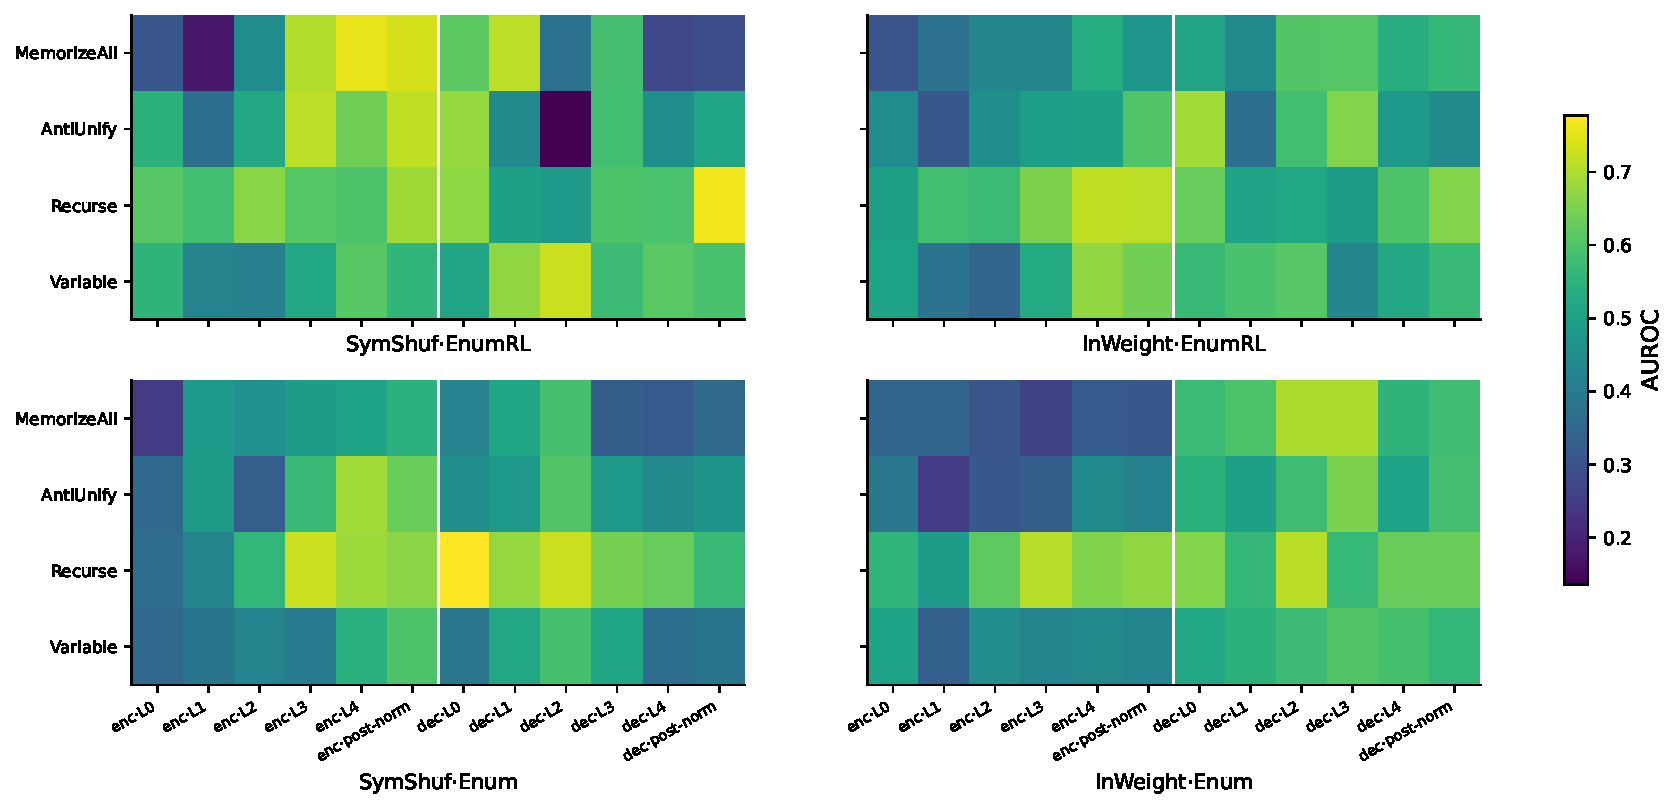
\includegraphics[width=0.9\textwidth]{media/probing/heatmap_layers_grid.pdf}
    \caption{Per-layer AUROC grids for each model and primitive, on a shared colour scale across panels so that within- and across-model comparisons remain commensurable.}
    \label{fig:heatmap}
\end{figure}

\end{document}
